\documentclass[red]{beamer}
\usepackage{beamerthemebars} 
% Other themes include: beamerthemesplit, beamerthemebars, beamerthemelined, 
%                       beamerthemetree, beamerthemetreebars  
%\addbibresource{mini_presentation.bib}

\title{On Choosing a Task Assignment Policy for a Distributed Server System\cite{paper}}    
\author{Ferhat Elmas}                 
\institute{Performance Evaluation Mini Project}      
\date{\today}                    

\begin{document}

\begin{frame}
  \titlepage
\end{frame}

\section[Outline]{}

\begin{frame}
  \tableofcontents[hideallsubsections]
\end{frame}

\section{Introduction}

\subsection{Definition}
\begin{frame}
  \frametitle{Introduction}   

\begin{itemize}
\item A task assignment policy for a distributed server system that composed of multiple hosts which process tasks in FCFS.
\end{itemize}

  \begin{enumerate}
  \item<1-> \textbf{Random}: One of the hosts is randomly chosen. Each of host has an equal probability. 
  \item<2-> \textbf{Round Robin}: Tasks are assigned to hosts in cyclic fashion.
  \item<3-> \textbf{Dynamic}: The task is assigned to the host that has minimum expected waiting time.
  \item<4-> \textbf{Size Based}: Task size is partitioned and tasks that are in a certain range are assigned to a particular host.
  \end{enumerate}

\end{frame}

\subsection{Motivation}

\begin{frame}
  \frametitle{Motivation}  

  \begin{itemize}
  \item<1-> Task Assignment Policies are studied extensively
    \begin{itemize}
  	  \item<1-> Task Size is modelled in exponential 
 	  \item<1-> Exponential is a poor model
    \end{itemize}
  \item<2-> Real task sizes show heavy tail property
    \begin{itemize}
  	  \item<2-> Very small fraction of task makes nearly half of the load
 	  \item<2-> $Pr(X > x) \sim X^{-a}$ where $ 0 \le a \le 2$
 	  \item<2-> Lower \textit{a} implies more variable task size
    \end{itemize}
  
  \end{itemize}
\end{frame}

\begin{frame}
	\frametitle{Motivation - Real Values}
	
	\begin{center}

	\begin{tabular}{|c|c|}
	\hline
		\textbf{\textit{Task Description}}    & \textbf{\textit{a}}\\		
	\hline
		Unix CPU requirements at BellCore     & $ [ 1, 1.25 ]$ \\
	\hline
		Unix CPU requirements at Berkeley     & $ \sim 1 $ \\
	\hline
		Size of files transferred through Web & $ [ 1.1, 1.3 ]$ \\
	\hline
		Size of FTP transfers in the internet & $ [ 0.9, 1.1 ]$ \\
	\hline
		I/O Times & $ \sim 0 $ \\
	\hline
	\end{tabular}
	\end{center}
	
    \begin{itemize}
	\item That's why \textit{Microsoft Windows} can't predict 
	  \begin{itemize}
		\item How much time is left while moving, copying files
	  \end{itemize}		
	\end{itemize}	
\end{frame}

\begin{frame}
	\frametitle{Motivation - Comparison of Exponential and Pareto}
	
  \begin{columns}[c]
  	\column{2in}  % slides are 3in high by 5in wide
  	\framebox{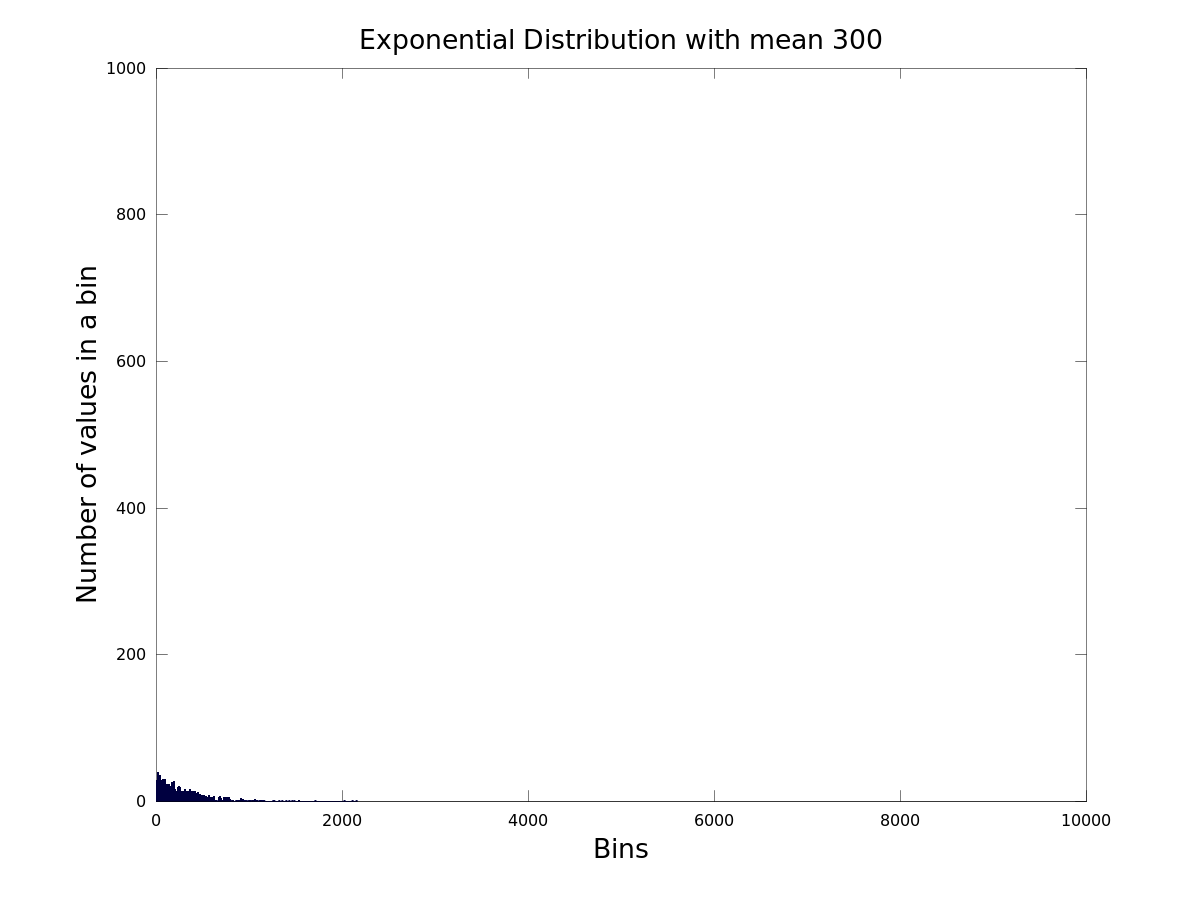
\includegraphics[scale=0.13]{alfa/randoms/exponential_hist}}
  	\column{2in}
  	\framebox{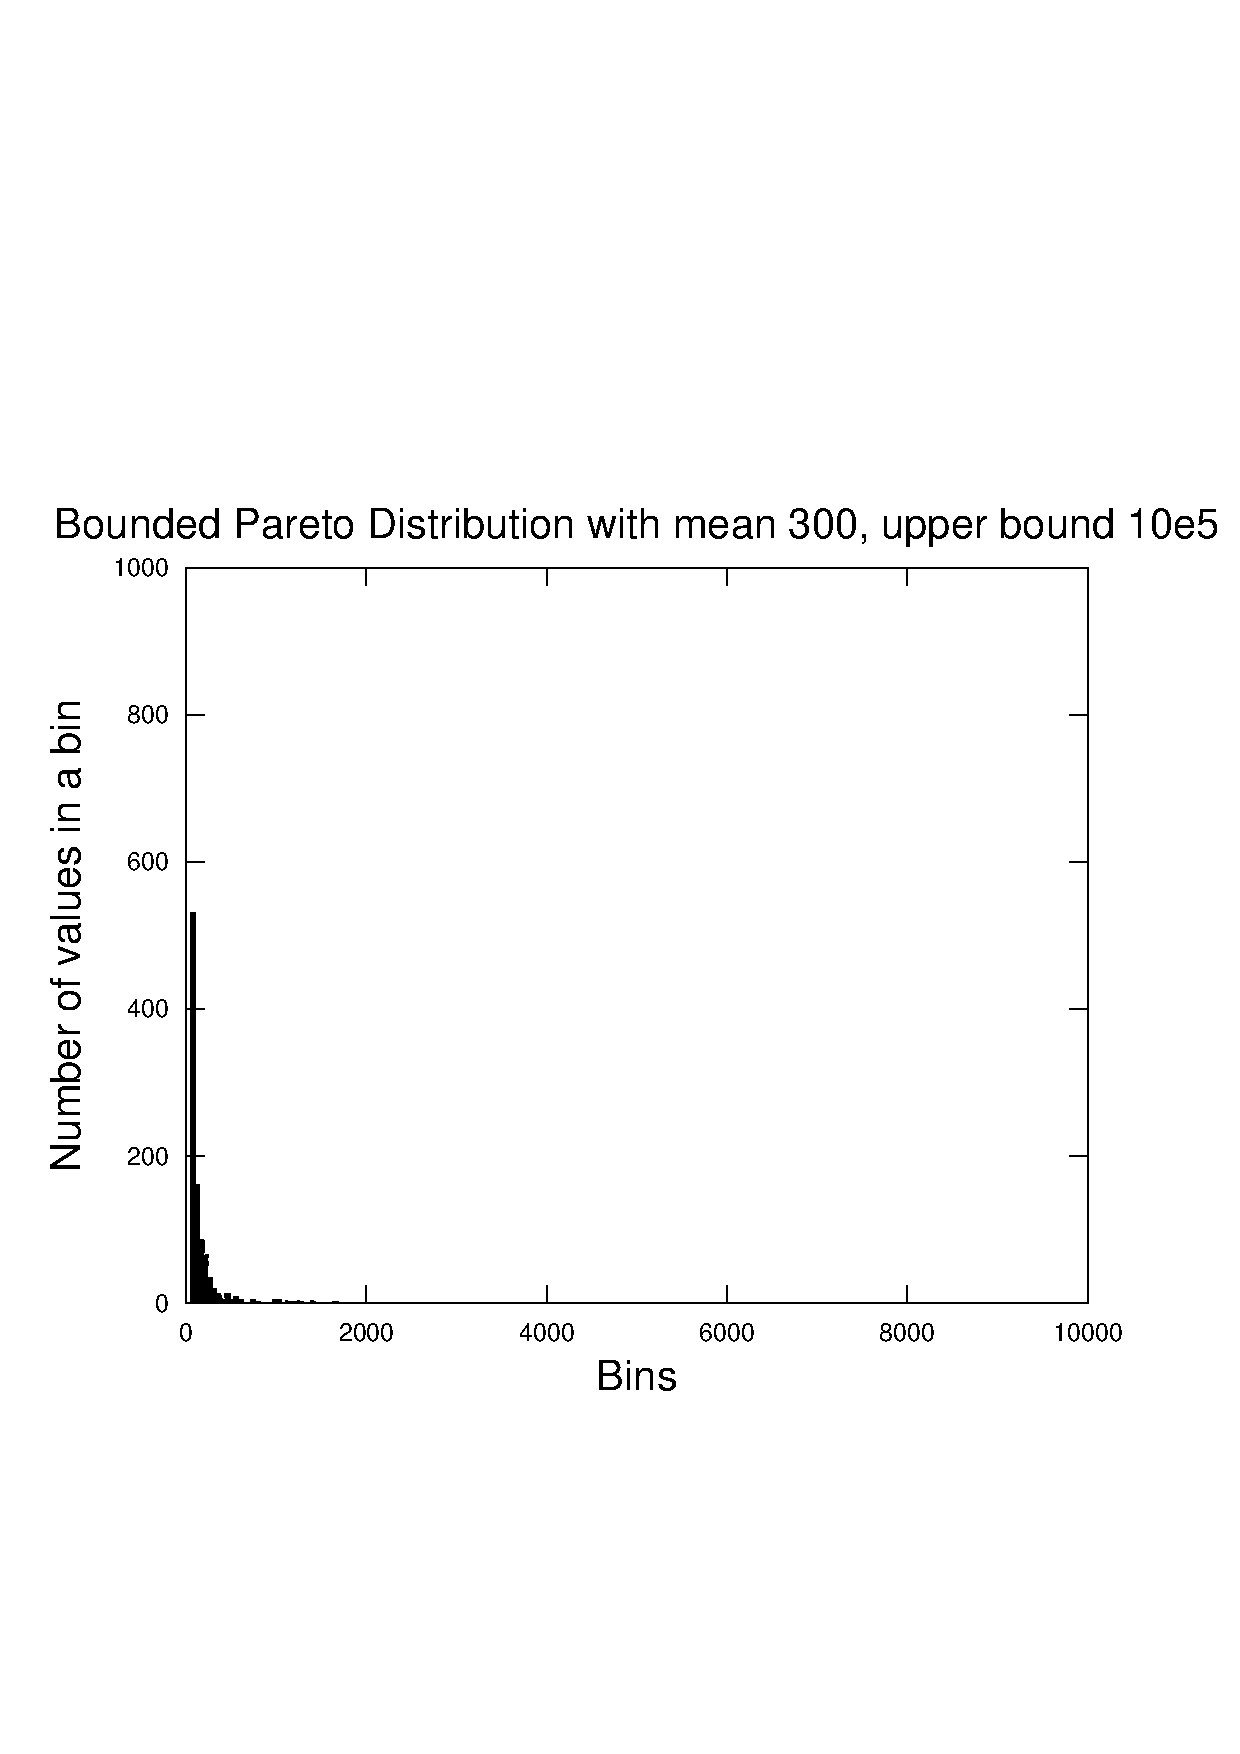
\includegraphics[scale=0.13]{alfa/randoms/pareto_hist}}
  \end{columns}
	
\end{frame}

\section{Model}
\subsection{Assumptions}
\begin{frame}
  \frametitle{Assumptions}   % Insert frame title between curly braces
  \begin{itemize}
 	\item<1-> Task Size is known in advance
	\item<2-> Service time is equal to size of task, no scheduling overhead
	\item<3-> CPU is the only resource
	\item<4-> Hosts in the server are identical
	\item<5-> Task is assigned to a host as soon as it arrives.
	\item<6-> Execution is in FCFS and non-preemptive
  \end{itemize}
\end{frame}
\note{The end}       % Add notes to yourself that will be displayed when
		     % typeset with the notes or notesonly class options
\subsection{System Model}
\begin{frame}
	\frametitle{System Model}
	
  \begin{itemize}
 	\item<1-> Task arrival rate is poisson.
	\item<2-> Task size is bounded pareto distribution.
	\item<3-> Defined as $ B(k, p, a) $
		\begin{itemize}	
			\item $ P(x) = \frac{a \cdot k^a \cdot x^{-a-1}}{1 - {\frac{k}{p}}^a} $ where $ k <= x <= p $
		\end{itemize}
	\item<4-> $ a $ shape parameter and controls variance
		\begin{itemize}
			\item Smaller $ a \rightarrow $ Higher variance
			\item Varies in range of $ [1, 2] $
		\end{itemize}	
  \end{itemize}
 
\end{frame}

\subsection{Performance}
\begin{frame}
	\frametitle{Performance Measures}
	
	\begin{itemize}
		\item<1-> Average Waiting Time
		\item<2-> Average Slow Down
			\begin{itemize}
				\item $ \frac{Waiting Time}{Task Size} $
			\end{itemize}
	\end{itemize}

\end{frame}

\section{Simulation}
\subsection{Input Parameters}
\begin{frame}
	\frametitle{System Parameters}
	
	\begin{itemize}
		\item<1-> Number of Servers
		\item<2-> Load
		\item<3-> $a$ shape parameter of pareto distribution
			\begin{itemize}
			\item while $a$ is changing, $k$ is adjusted to keep the mean same
			\end{itemize}
	\end{itemize}

\end{frame}

\subsection{Schedule}
\begin{frame}
	\frametitle{Schedule Algorithms}
	
	\begin{itemize}
		\item<1-> \textbf{Random}:
			\begin{itemize}
			\item Host $h \leftarrow $ Task $ t $ where $ \frac{h}{|H|} \le u < \frac{h+1}{|H|}$ where $ u \sim U[0, 1] $ 
			\end{itemize}
		\item<2-> \textbf{Round Robin}:
			\begin{itemize}
			\item Host $h \leftarrow $ Task $ t $ where $ t \equiv h \pmod{|H|} $
			\end{itemize}
		\item<3-> \textbf{Dynamic}:
			\begin{itemize}
			\item Host $h \leftarrow $ Task $ t $ where $ h = getHostWithMinTaskQueue()$
			\end{itemize}
		\item<4-> \textbf{Size Based}:
			\begin{itemize}
			\item Host $h \leftarrow $ Task $ t $ where $ bounds[h] \le t.size < bounds[h+1] $
			\end{itemize}
		
	\end{itemize}

\end{frame}

\begin{frame}
	\frametitle{Schedule Algorithms - Size Based Bound Calculation}
	
	Bounds $ x_i $ \vspace{0.4cm} \linebreak 
	$ k = x_0 < x_1 < x_2 < \dots < x_{h-1} < x_h = p $ \linebreak
	$ \int\limits_{k=x_0}^{x_1} x \cdot \, dF(x) =  \int\limits_{x_1}^{x_2} x \cdot \, dF(x) = \cdots =  \int\limits_{x_{h-1}}^{x_h=p} x \cdot \, dF(x) = \frac{\mu}{h} = \frac{\int\limits_{k}^{p} x \cdot \, dF(x)}{h} $			
\end{frame}

\subsection{Input Values}
\begin{frame}
	\frametitle{Simulation Values}
	\vspace{-.3cm}
	\begin{itemize}
	\item To study variance
		\begin{itemize}
		\item $ a \leftarrow (1.1 + 0.1 \cdot step) $ where $ 0 \le step < 9 $ 
		\end{itemize}
	\item $ p = 100000, \mu = 300 $
		\begin{itemize}
		\item $k$ is adjusted \linebreak
		\begin{tabular}{cc}
			$k = 51 \leftarrow a = 1.1$ \\
			$k = 65 \leftarrow a = 1.2$ \\
			$k = 78 \leftarrow a = 1.3$ \\
			$k = 91 \leftarrow a = 1.4$	\\		
			$k = 103 \leftarrow a = 1.5$ \\
			$k = 114 \leftarrow a = 1.6$ \\
			$k = 125 \leftarrow a = 1.7$ \\
			$k = 134 \leftarrow a = 1.8$ \\
			$k = 142 \leftarrow a = 1.9$ \\
		\end{tabular}
		\end{itemize}
	\item Load is fixed at $0.8$ so arrival rate is
	\begin{itemize}
		\item $Rate = \frac{h \cdot load}{\mu}$
	\end{itemize}
	\end{itemize}		
	
\end{frame}

\begin{frame}
	\frametitle{Simulation Values - 2}
	
	\begin{itemize}
	\item Number of arrival tasks 
		\begin{itemize}
		\item Sufficient condition to finish simulation
		\item $ t = 10^7$
		\end{itemize}
	\item Number of Runs
		\begin{itemize}
		\item Required condition to get confidence
		\item $ r = 100$
		\end{itemize}
	\item Steady state
		\begin{itemize}
		\item Required condition to sense heavy tail
		\item After $2*10^6$ task arrivals, 20\% of all tasks
		\end{itemize}
	\end{itemize}
\end{frame}

\section{Simulation Results}

\subsection{Overall Results}
\begin{frame}
\frametitle{Average Time Comparison to Exponential}

\hspace*{-0.8cm}
\begin{tabular}{|c|c|c|c|c|}
\hline
&\multicolumn{2}{|c|}{Exponential} & \multicolumn{2}{|c|}{Bounded Pareto($a=1.1$)} \\
\hline
Policy & Waiting Time & SlowDown & Waiting Time & SlowDown \\
\hline
Random & 1262.5670 & 4.2152 & 19890.4074 & 66.6756 \\
\hline
Round Robin & 630.2895 & 2.1033 & 19103.7297 & 64.1288 \\
\hline
Dynamic & 122.1085 & 0.4078 & 924.5439 & 3.0929 \\
\hline
Size Based & 693.9924 & 2.3162 & 650.5760	& 2.1863 \\
\hline
\end{tabular}

\end{frame}

\subsection{Graphs}
\begin{frame}
\vspace{-.05cm}
\hspace{.2cm}\framebox{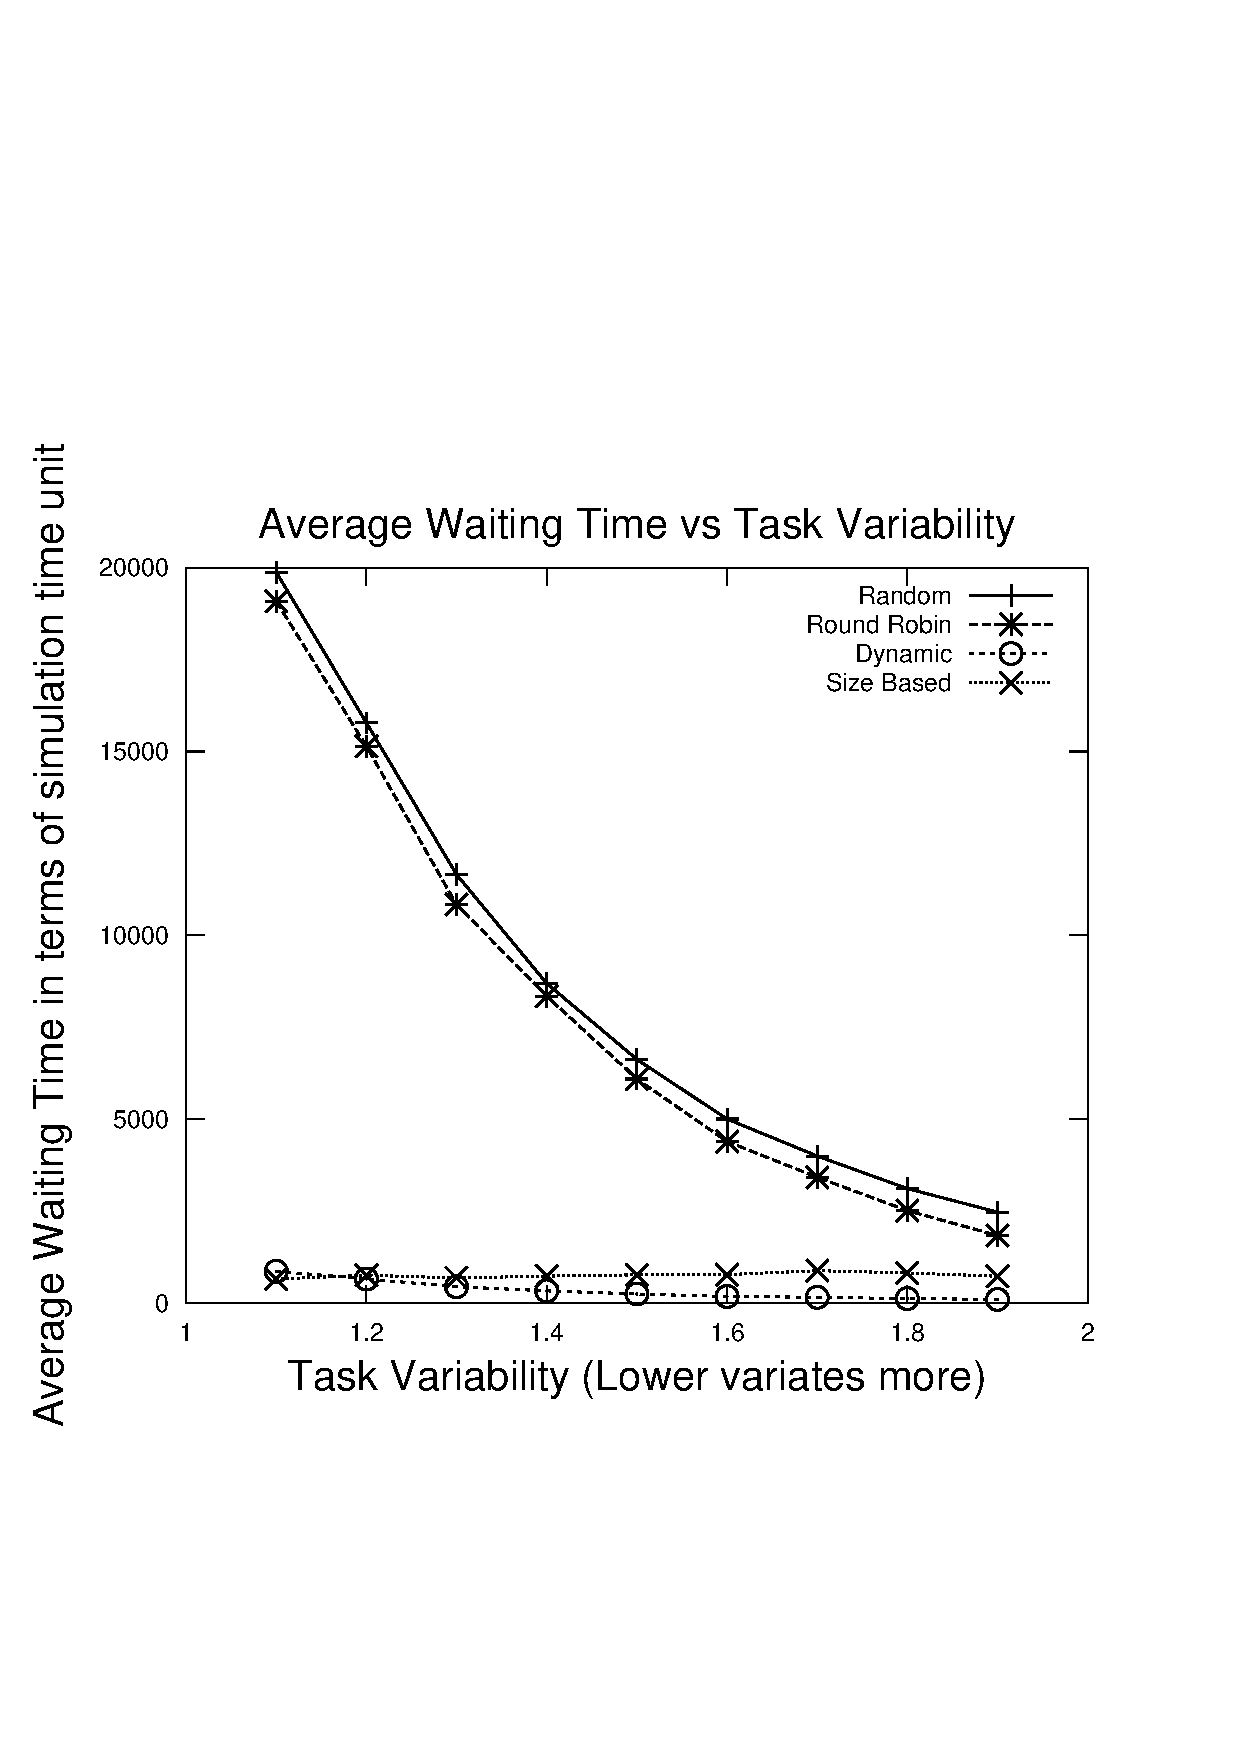
\includegraphics[scale=0.24]{alfa/graphs/paretoAverageWaitingTime}}
\end{frame}

\begin{frame}
\vspace{-.05cm}
\hspace{.2cm}\framebox{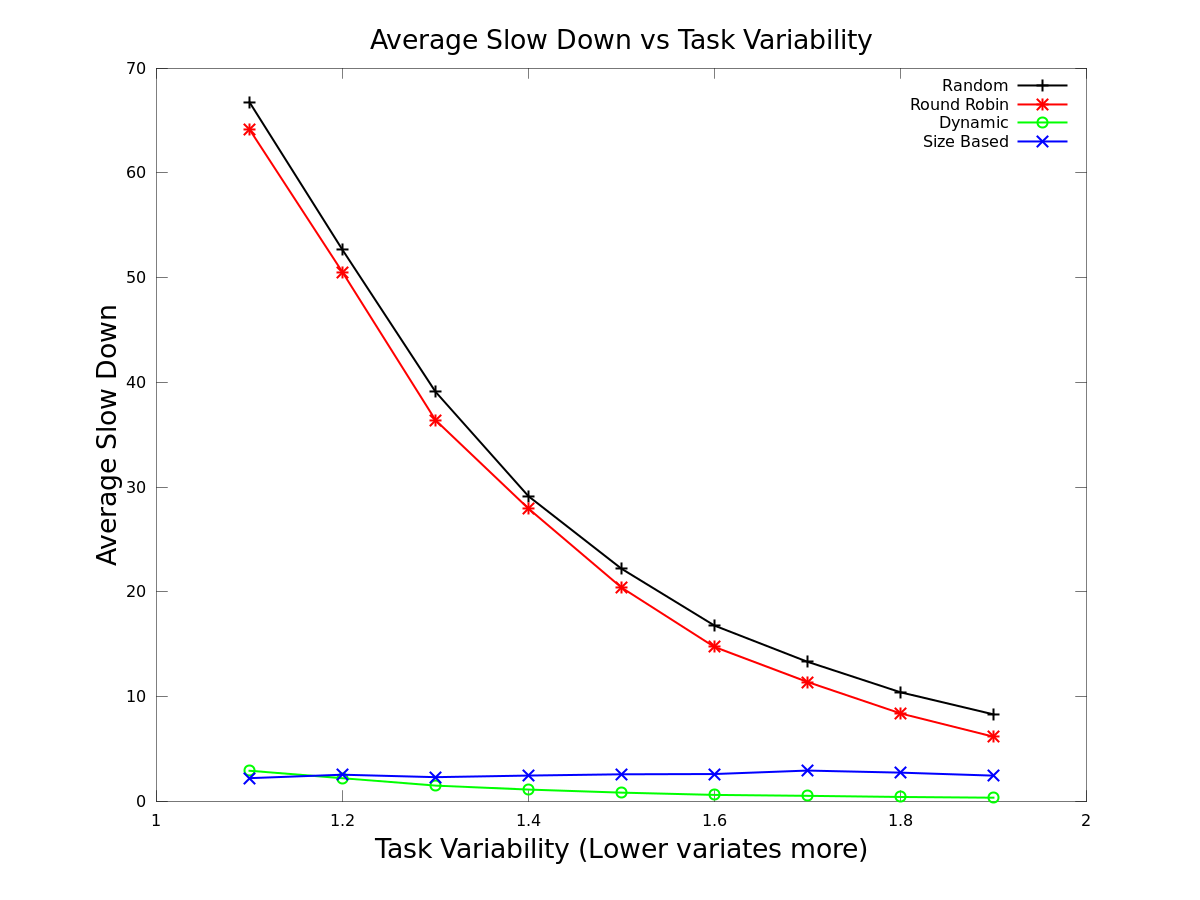
\includegraphics[scale=0.24]{alfa/graphs/paretoAverageSlowDown}}
\end{frame}

\subsection{Confidence Intervals}
\begin{frame}
\frametitle{Confidence Intervals}

\vspace{-1cm}
\begin{itemize}
\item 100 runs
\end{itemize}
\vspace{.5cm}

\hspace*{1cm}
\begin{tabular}{|c|c|c|}
\hline
\multicolumn{3}{|c|}{Exponential} \\
\hline
Policy & Lower Bound & Upper Bound \\
\hline
RANDOM & 1249.26593	& 1263.79357 \\
\hline
ROUND ROBIN & 622.54191	& 632.53330 \\
\hline
DYNAMIC & 121.35404	& 123.49327 \\
\hline
SIZE BASED: & 684.83063	& 696.14331 \\
\hline
\end{tabular}
\end{frame}

\begin{frame}
\frametitle{Confidence Intervals - 2}

\vspace{-.2cm}
\begin{itemize}
\item 100 runs
\end{itemize}
\vspace{.3cm}

\hspace*{1cm}
\begin{tabular}{|c|c|c|}
\hline
\multicolumn{3}{|c|}{Bounded Pareto - Random Policy} \\
\hline
\textit{a} & Lower Bound & Upper Bound \\
\hline
1.1 & 19428.98410 & 20437.87776 \\
\hline
1.2 & 14978.03231 & 16344.14195 \\
\hline
1.3 & 11089.38970 & 11961.20672 \\
\hline
1.4 & 8399.67174	 & 9102.56048 \\
\hline
1.5 & 6437.75149	 & 6913.98037 \\
\hline
1.6 & 4755.01100	 & 5129.61958 \\
\hline
1.7 & 3834.98348	 & 4183.03872 \\
\hline
1.8 & 2997.05842	 & 3172.11419\\
\hline
1.9 & 2324.65254	 & 2571.22622\\
\hline
\end{tabular}
\end{frame}

\begin{frame}
\frametitle{Confidence Intervals - 3}

\vspace{-.2cm}
\begin{itemize}
\item 100 runs
\end{itemize}
\vspace{.3cm}

\hspace*{1cm}
\begin{tabular}{|c|c|c|}
\hline
\multicolumn{3}{|c|}{Bounded Pareto - Round Robin Policy} \\
\hline
\textit{a} & Lower Bound & Upper Bound \\
\hline
1.1 & 18749.38675 & 20086.56348 \\
\hline
1.2 & 14379.42287 & 15940.56209 \\
\hline
1.3 & 10391.33202 & 11662.84883 \\
\hline
1.4 & 7853.41338	 & 8423.94786 \\
\hline
1.5 & 5795.79636	 & 6169.45627 \\
\hline
1.6 & 4178.87500	 & 4475.55269 \\
\hline
1.7 & 3159.88026	 & 3567.81041 \\
\hline
1.8 & 2373.26957	 & 2695.34599 \\
\hline
1.9 & 1718.44651	 & 2002.97348 \\
\hline
\end{tabular}
\end{frame}

\begin{frame}
\frametitle{Confidence Intervals - 4}

\vspace{-.2cm}
\begin{itemize}
\item 100 runs
\end{itemize}
\vspace{.3cm}

\hspace*{1cm}
\begin{tabular}{|c|c|c|}
\hline
\multicolumn{3}{|c|}{Bounded Pareto - Dynamic Policy} \\
\hline
\textit{a} & Lower Bound & Upper Bound \\
\hline
1.1 & 804.91955	& 985.55327 \\
\hline
1.2 & 619.41650	& 781.61605 \\
\hline
1.3 & 441.59131	& 530.17471 \\
\hline
1.4 & 339.75903	& 404.82852 \\
\hline
1.5 & 264.03451	& 285.85370 \\
\hline
1.6 & 205.73459	& 233.99490 \\
\hline
1.7 & 186.39173	& 194.75100 \\
\hline
1.8 & 154.97537	& 165.03551 \\
\hline
1.9 & 135.49628	& 141.11565 \\
\hline
\end{tabular}
\end{frame}

\begin{frame}
\frametitle{Confidence Intervals - 5}

\vspace{-.2cm}
\begin{itemize}
\item 100 runs
\end{itemize}
\vspace{.3cm}

\hspace*{1cm}
\begin{tabular}{|c|c|c|}
\hline
\multicolumn{3}{|c|}{Bounded Pareto - Size Based Policy} \\
\hline
\textit{a} & Lower Bound & Upper Bound \\
\hline
1.1 & 641.64633	& 688.31200 \\
\hline
1.2 & 665.11589	& 830.02852 \\
\hline
1.3 & 656.61129	& 730.20091 \\
\hline
1.4 & 707.65831	& 795.26298 \\
\hline
1.5 & 739.64542	& 827.10732 \\
\hline
1.6 & 730.64636	& 847.75423 \\
\hline
1.7 & 827.62977	& 948.85723 \\
\hline
1.8 & 810.10281	& 881.40799 \\
\hline
1.9 & 718.54123	& 756.09282 \\
\hline
\end{tabular}
\end{frame}

\subsection{Bin Graphs}
\begin{frame}
	\frametitle{Average Waiting Times by Task Size, a=1.1}
	\vspace{-.1cm}
\framebox{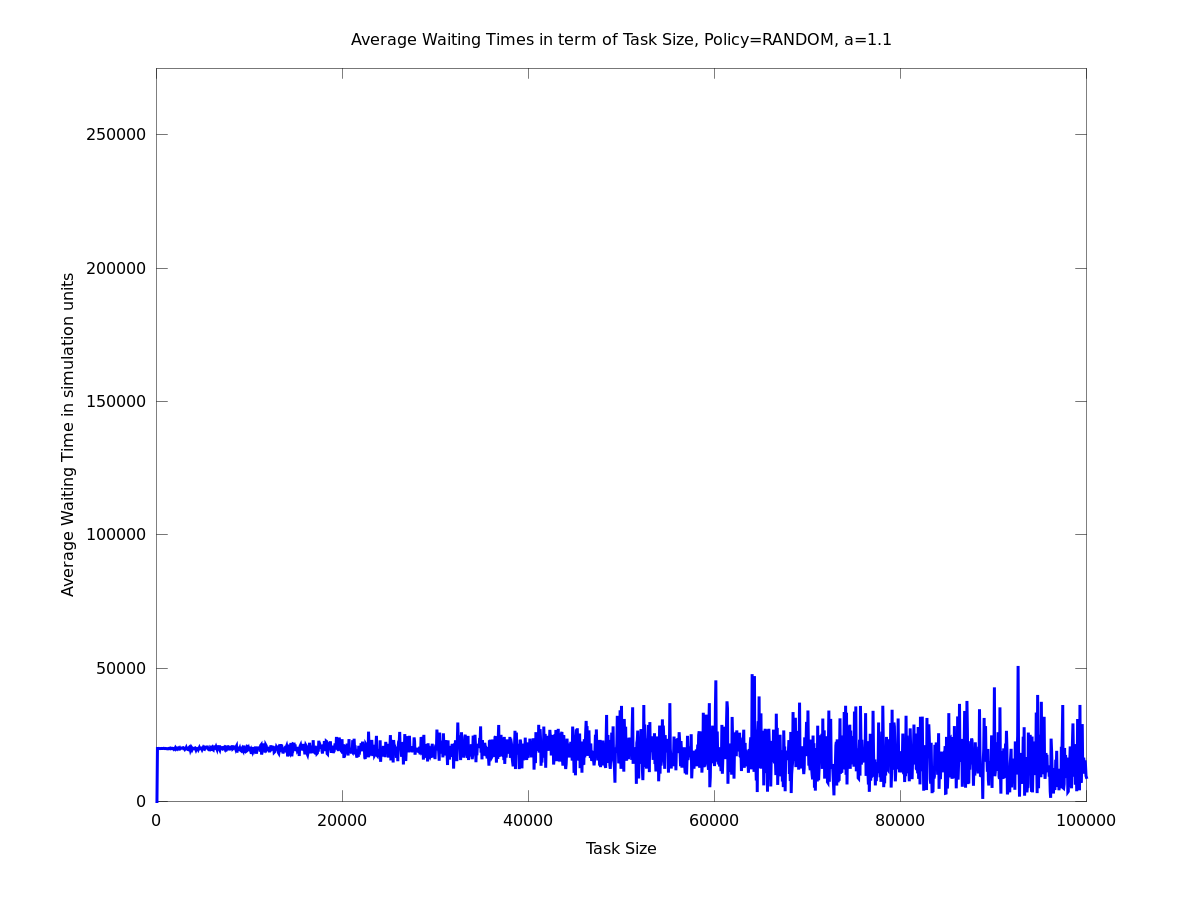
\includegraphics[scale=0.095]{alfa/graphs/binGraphs/waitingTime/bin1RandomWaitingTime}}
\framebox{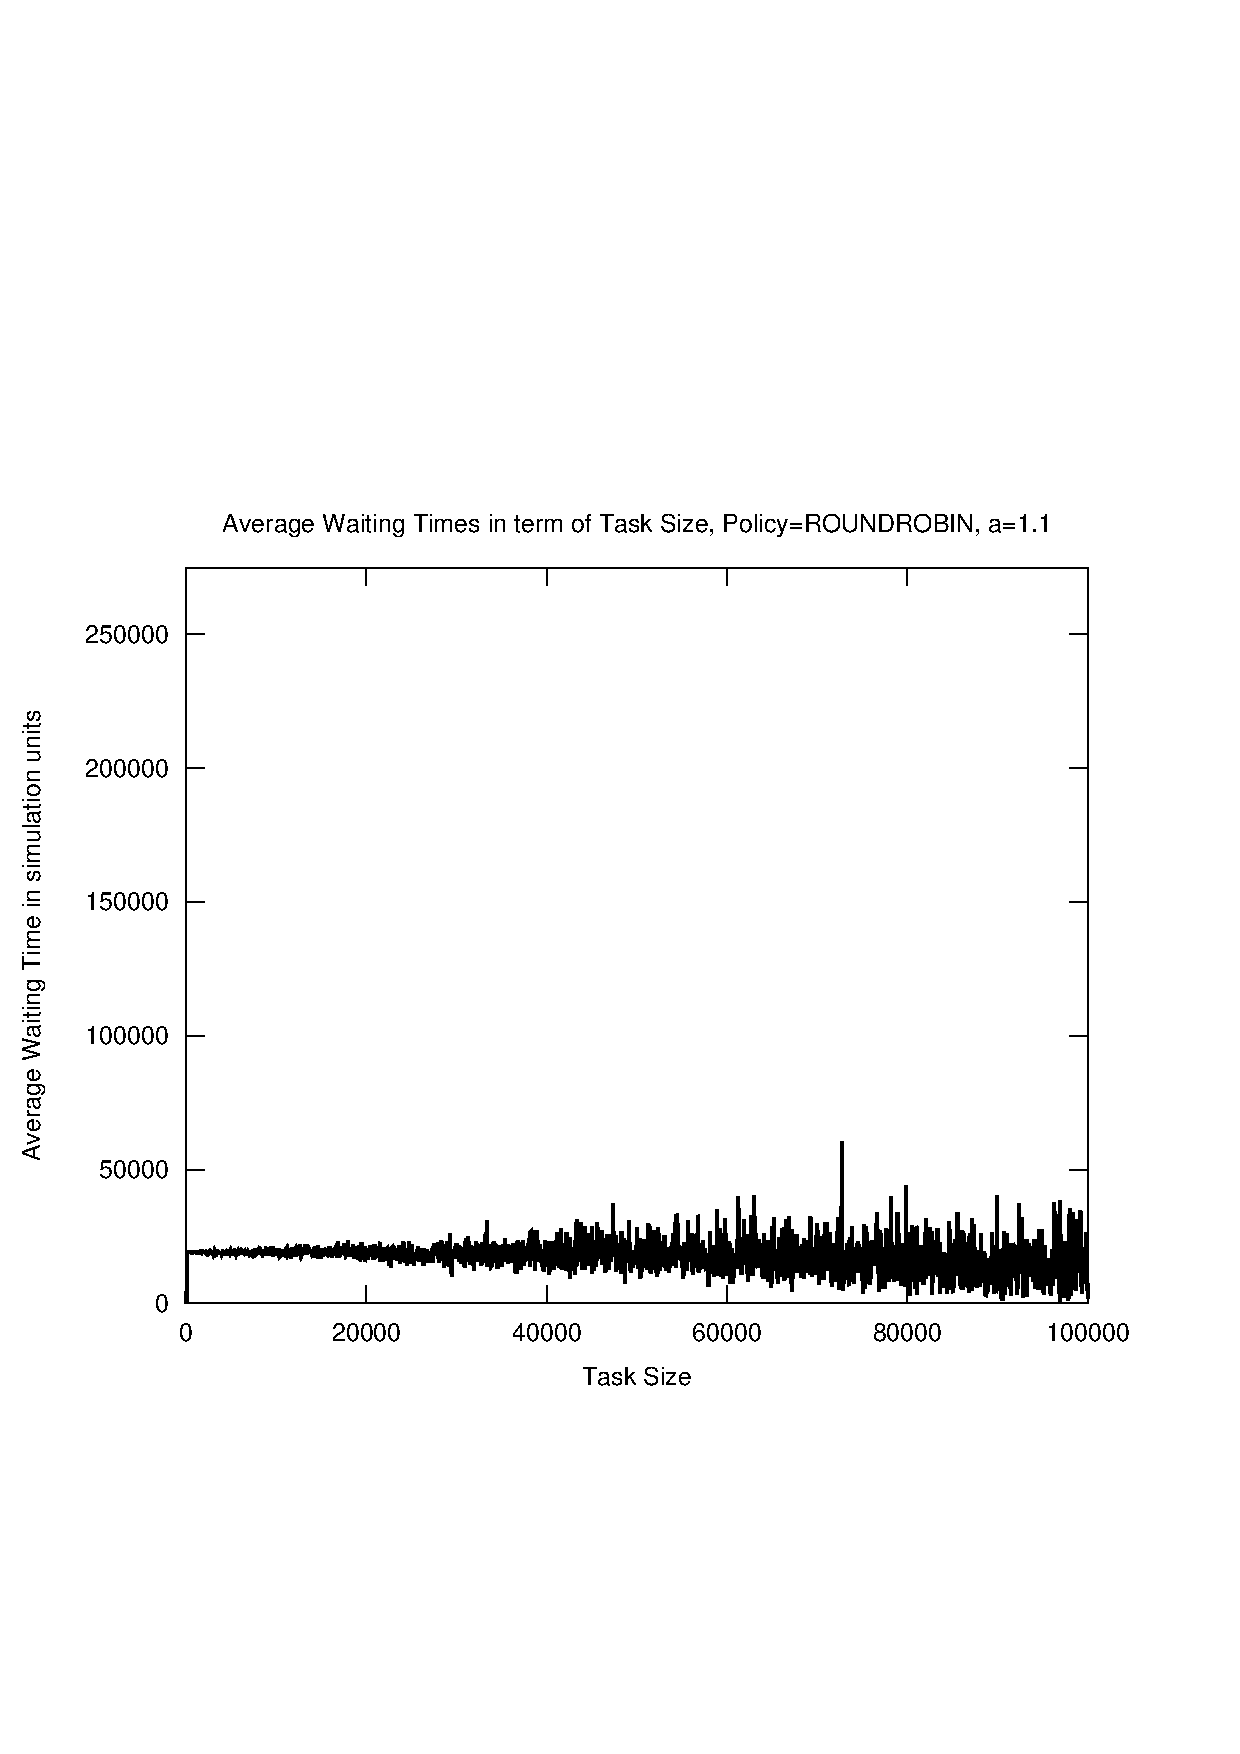
\includegraphics[scale=0.095]{alfa/graphs/binGraphs/waitingTime/bin1RoundWaitingTime}}
\framebox{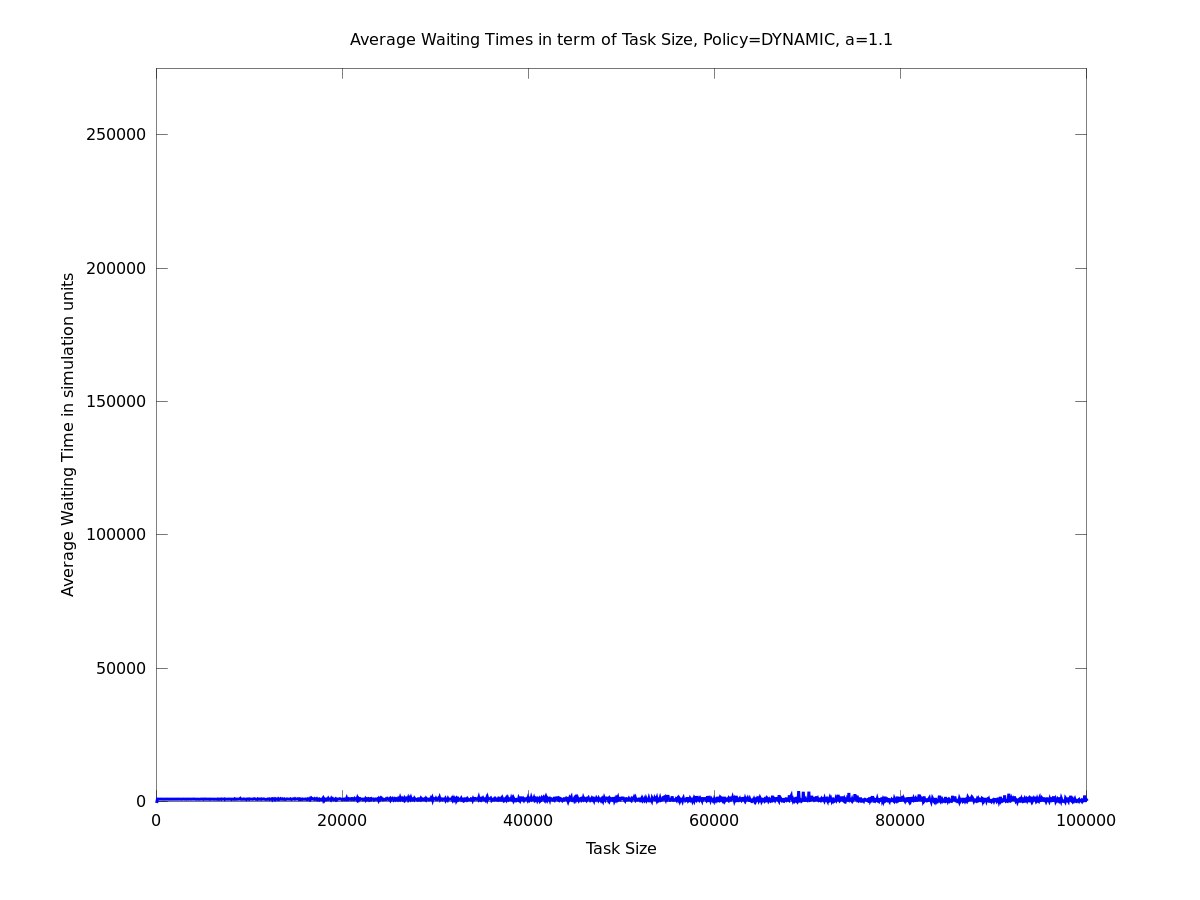
\includegraphics[scale=0.095]{alfa/graphs/binGraphs/waitingTime/bin1DynamicWaitingTime}}
\framebox{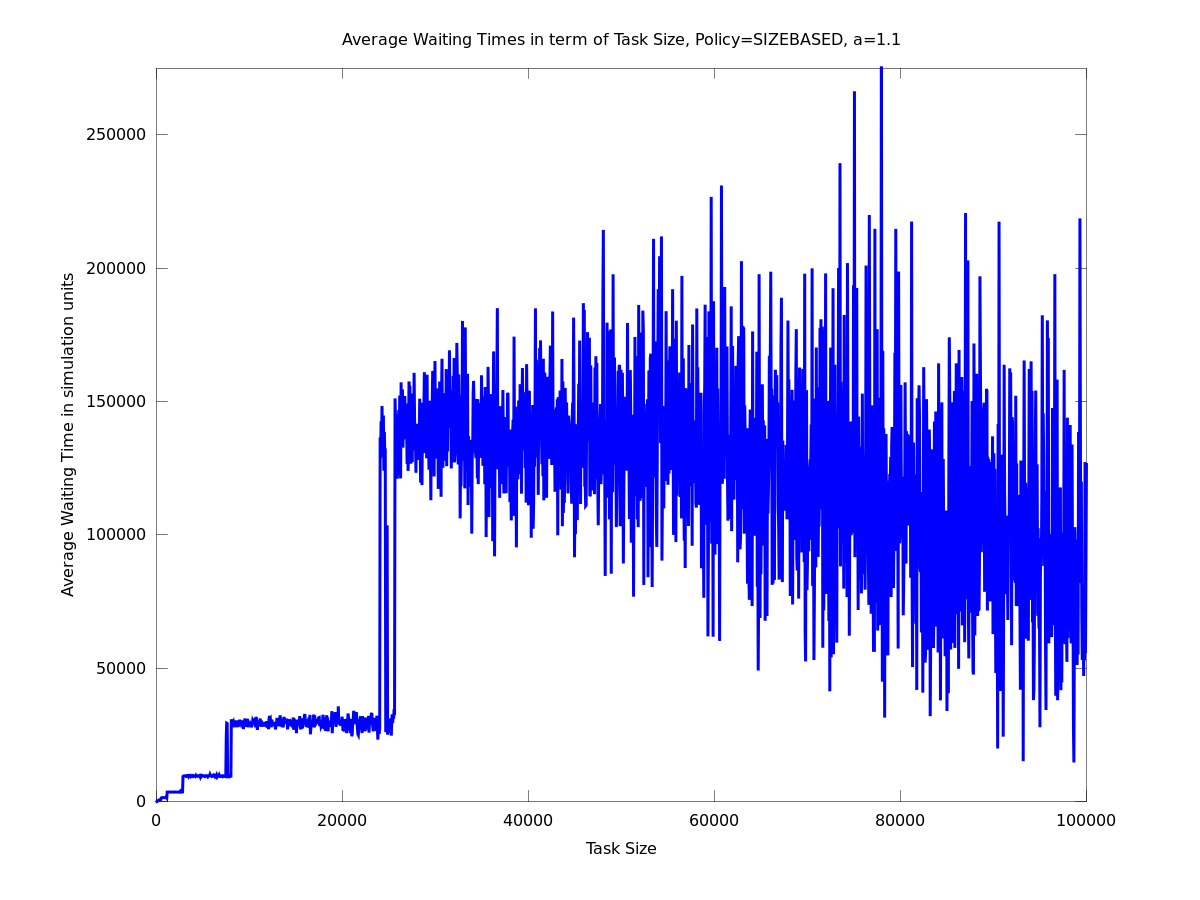
\includegraphics[scale=0.095]{alfa/graphs/binGraphs/waitingTime/bin1SizeWaitingTime}}
\end{frame}

\begin{frame}
	\frametitle{Average Waiting Times by Task Size, a=1.9}
	\vspace{-.1cm}
\framebox{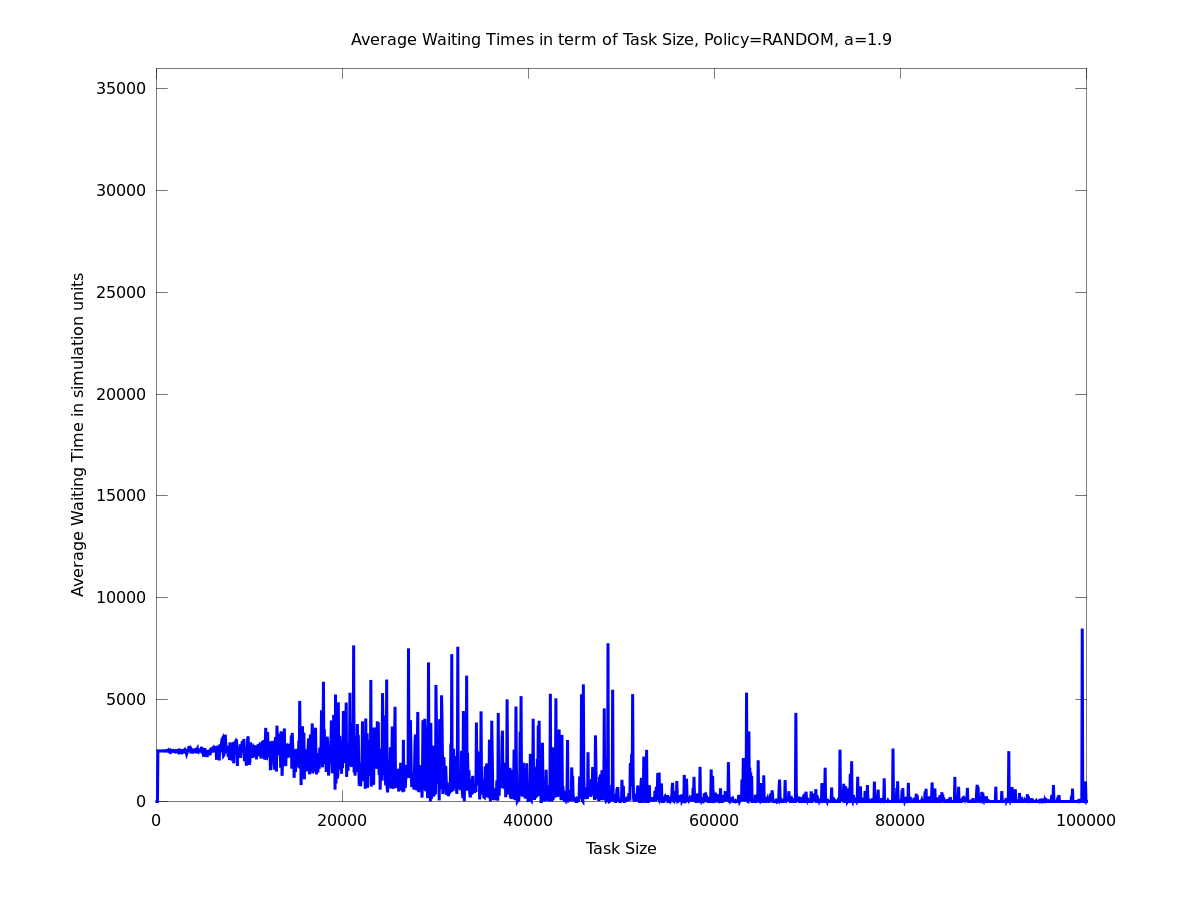
\includegraphics[scale=0.095]{alfa/graphs/binGraphs/waitingTime/bin9RandomWaitingTime}}
\framebox{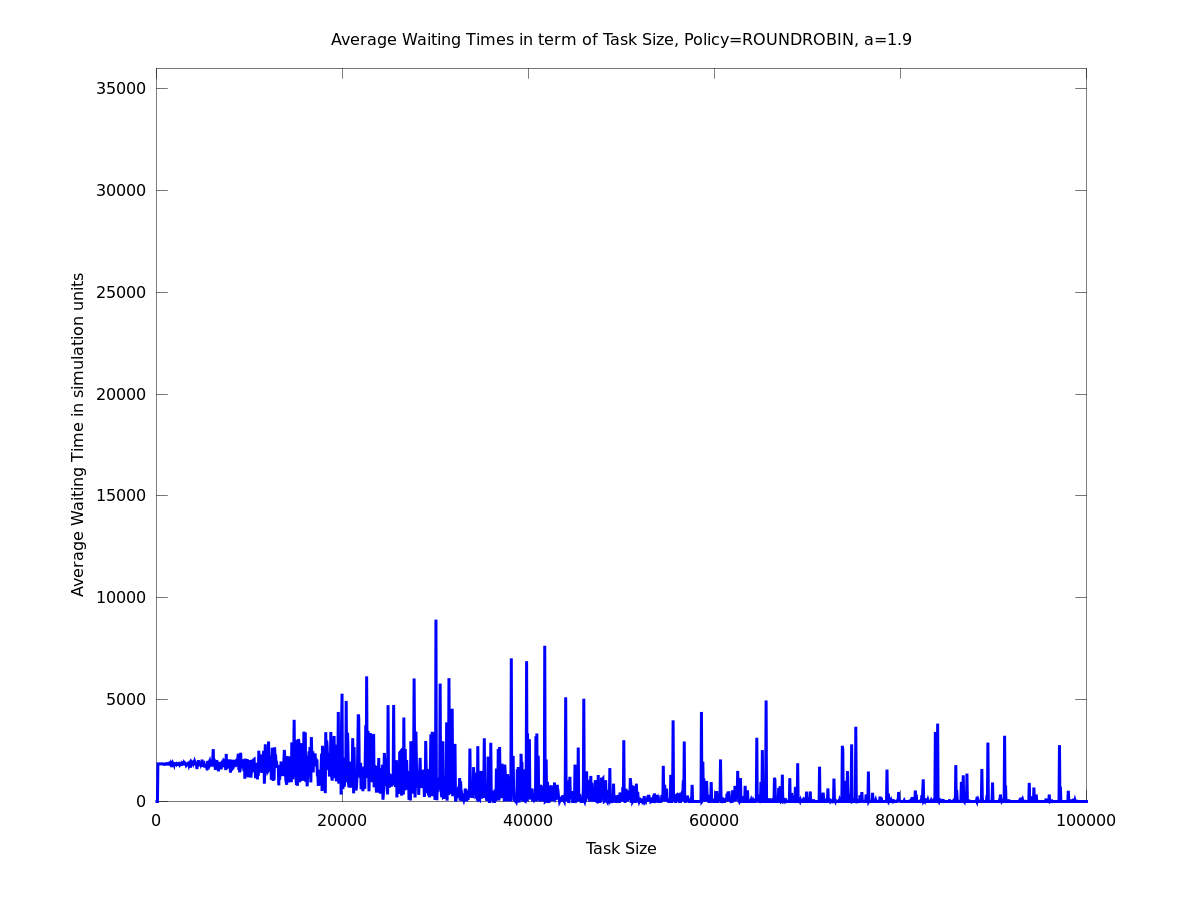
\includegraphics[scale=0.095]{alfa/graphs/binGraphs/waitingTime/bin9RoundWaitingTime}}
\framebox{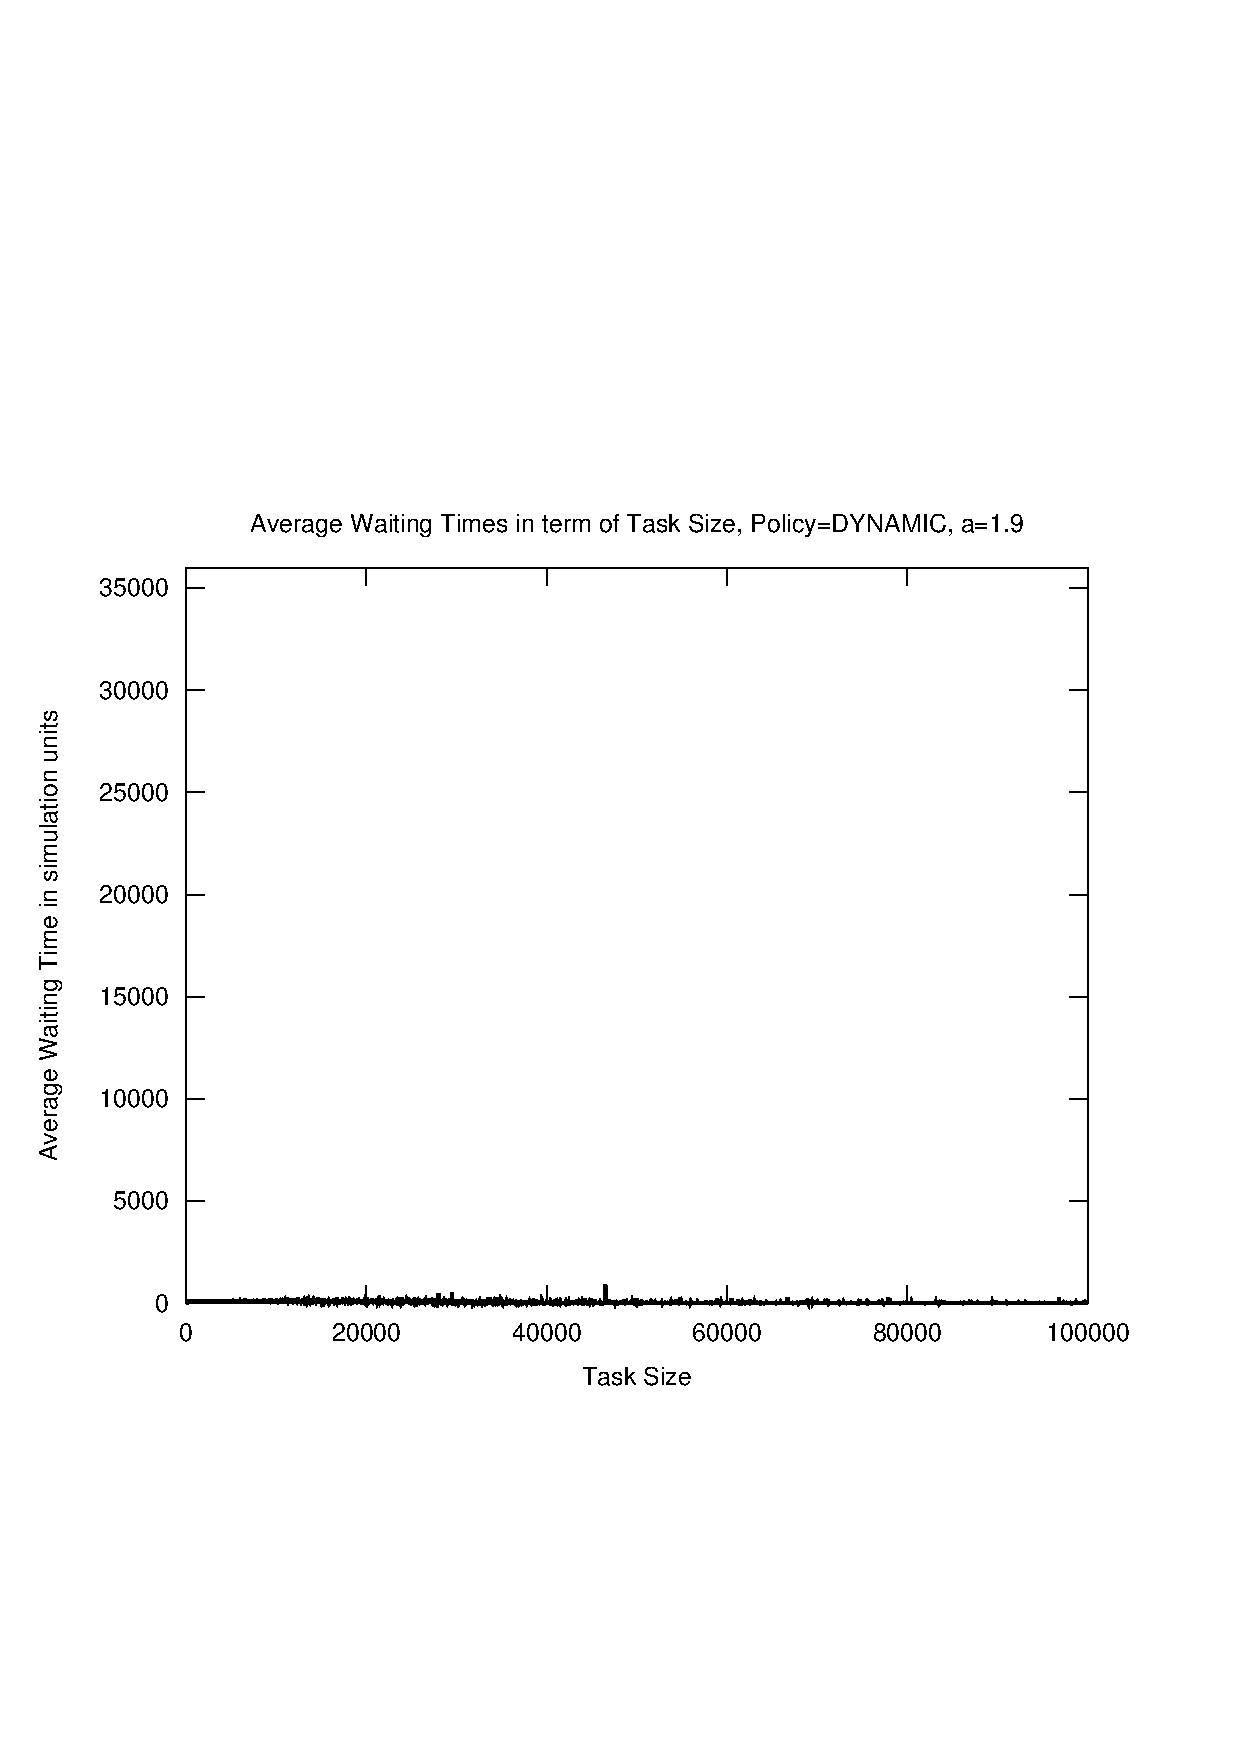
\includegraphics[scale=0.095]{alfa/graphs/binGraphs/waitingTime/bin9DynamicWaitingTime}}
\framebox{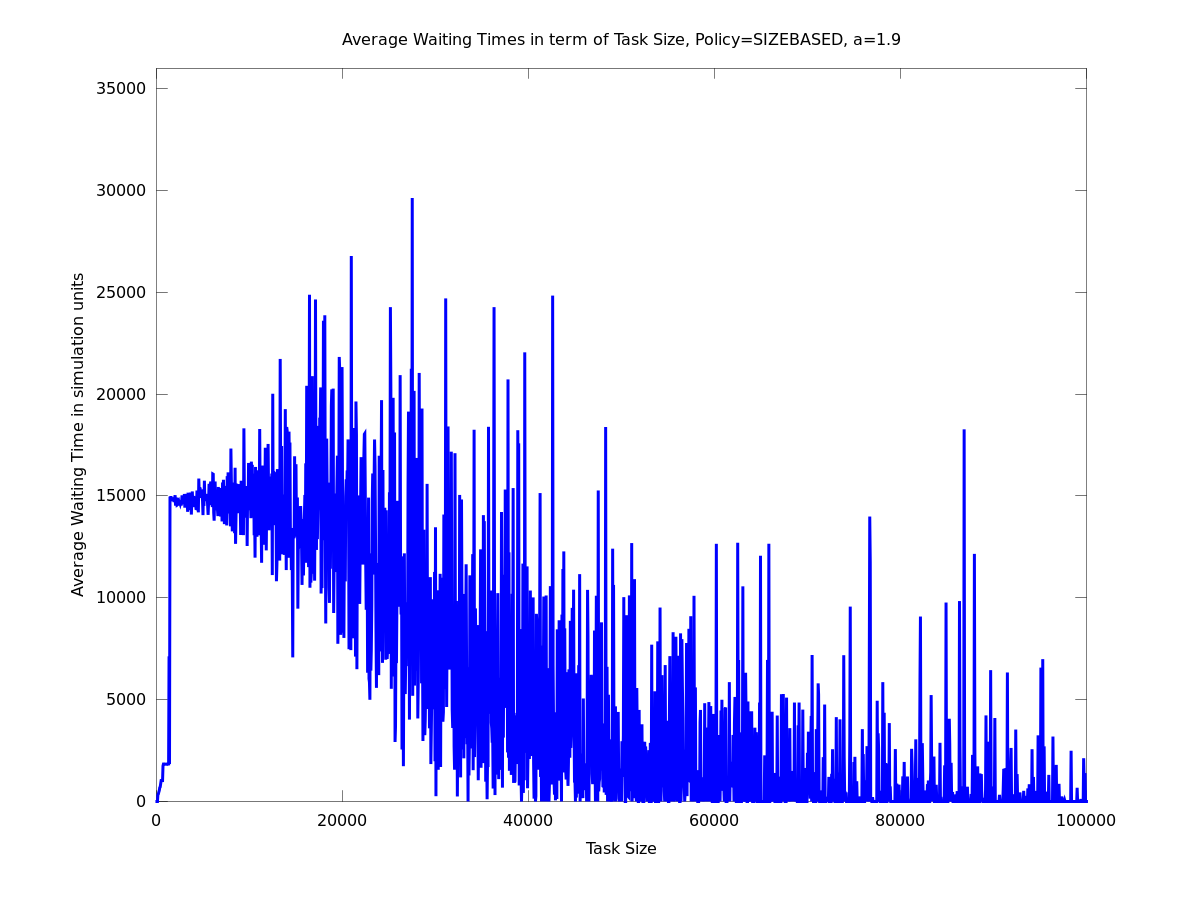
\includegraphics[scale=0.095]{alfa/graphs/binGraphs/waitingTime/bin9SizeWaitingTime}}
\end{frame}

\begin{frame}
	\frametitle{Average Slow Downs by Task Size, a=1.1}
	\vspace{-.1cm}
\framebox{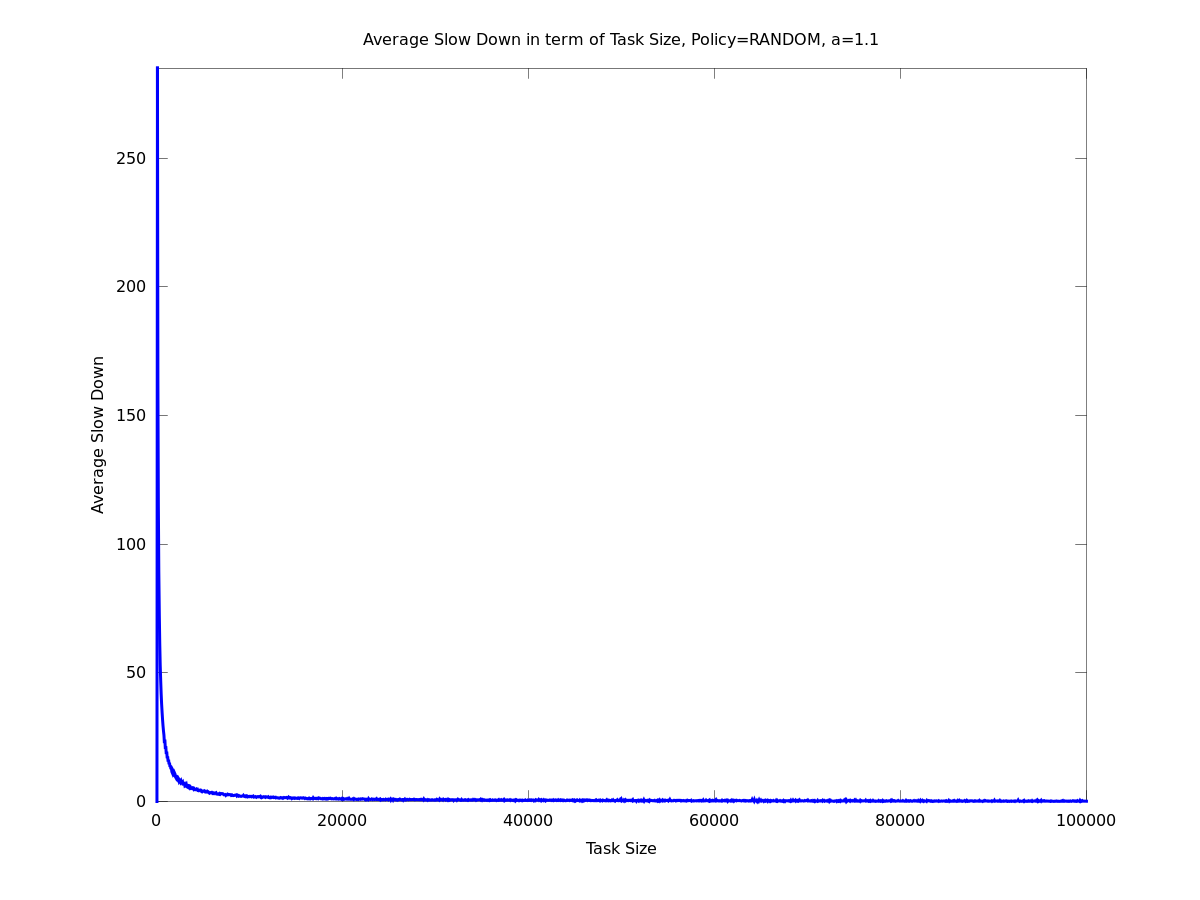
\includegraphics[scale=0.095]{alfa/graphs/binGraphs/slowDown/bin1RandomSlowDown}}
\framebox{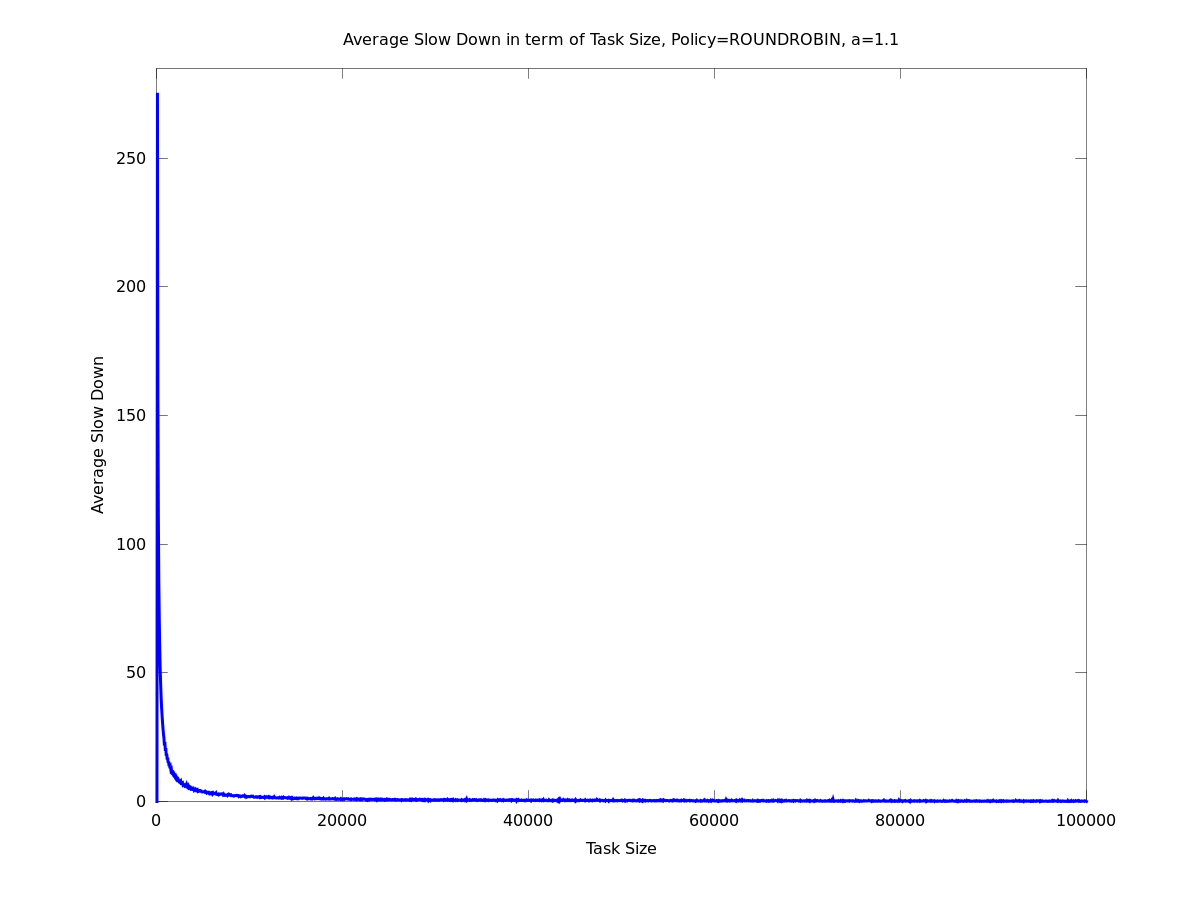
\includegraphics[scale=0.095]{alfa/graphs/binGraphs/slowDown/bin1RoundSlowDown}}
\framebox{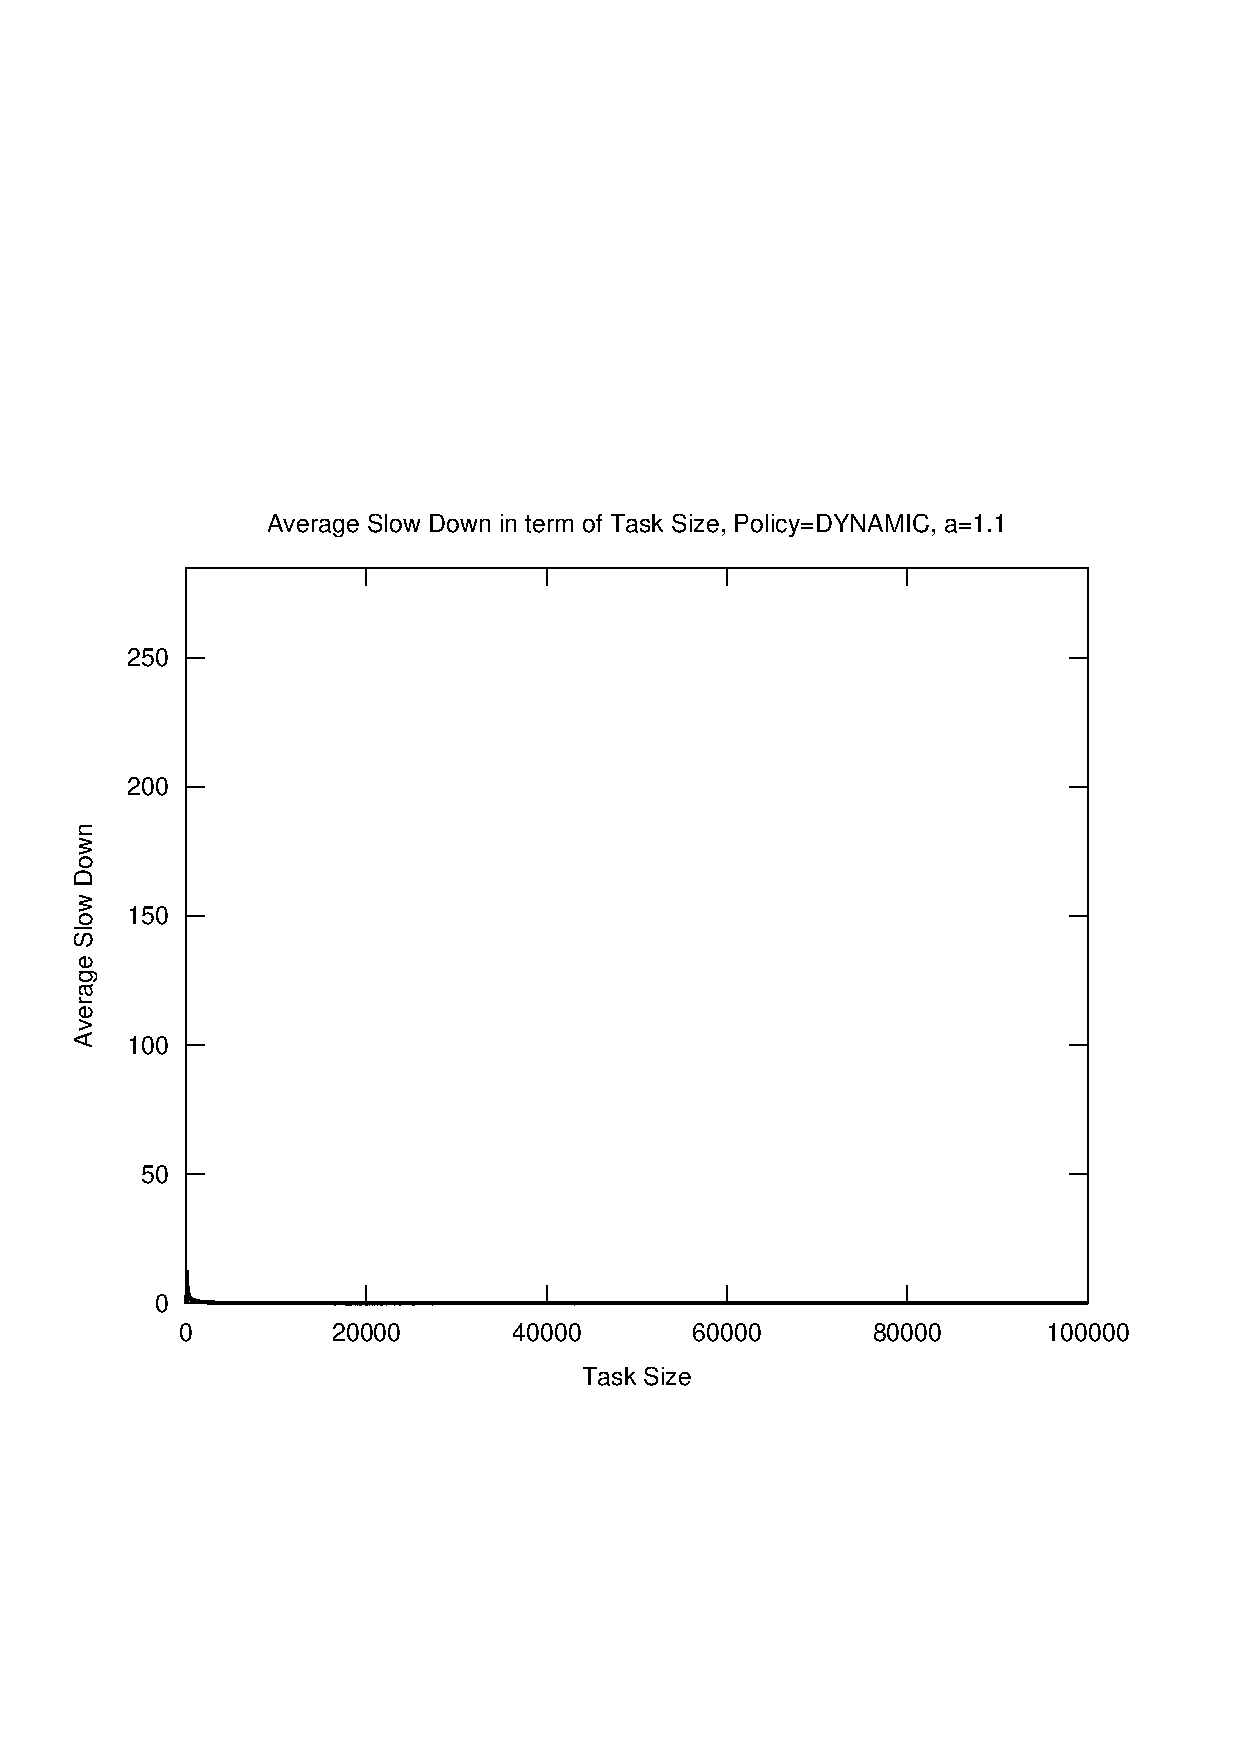
\includegraphics[scale=0.095]{alfa/graphs/binGraphs/slowDown/bin1DynamicSlowDown}}
\framebox{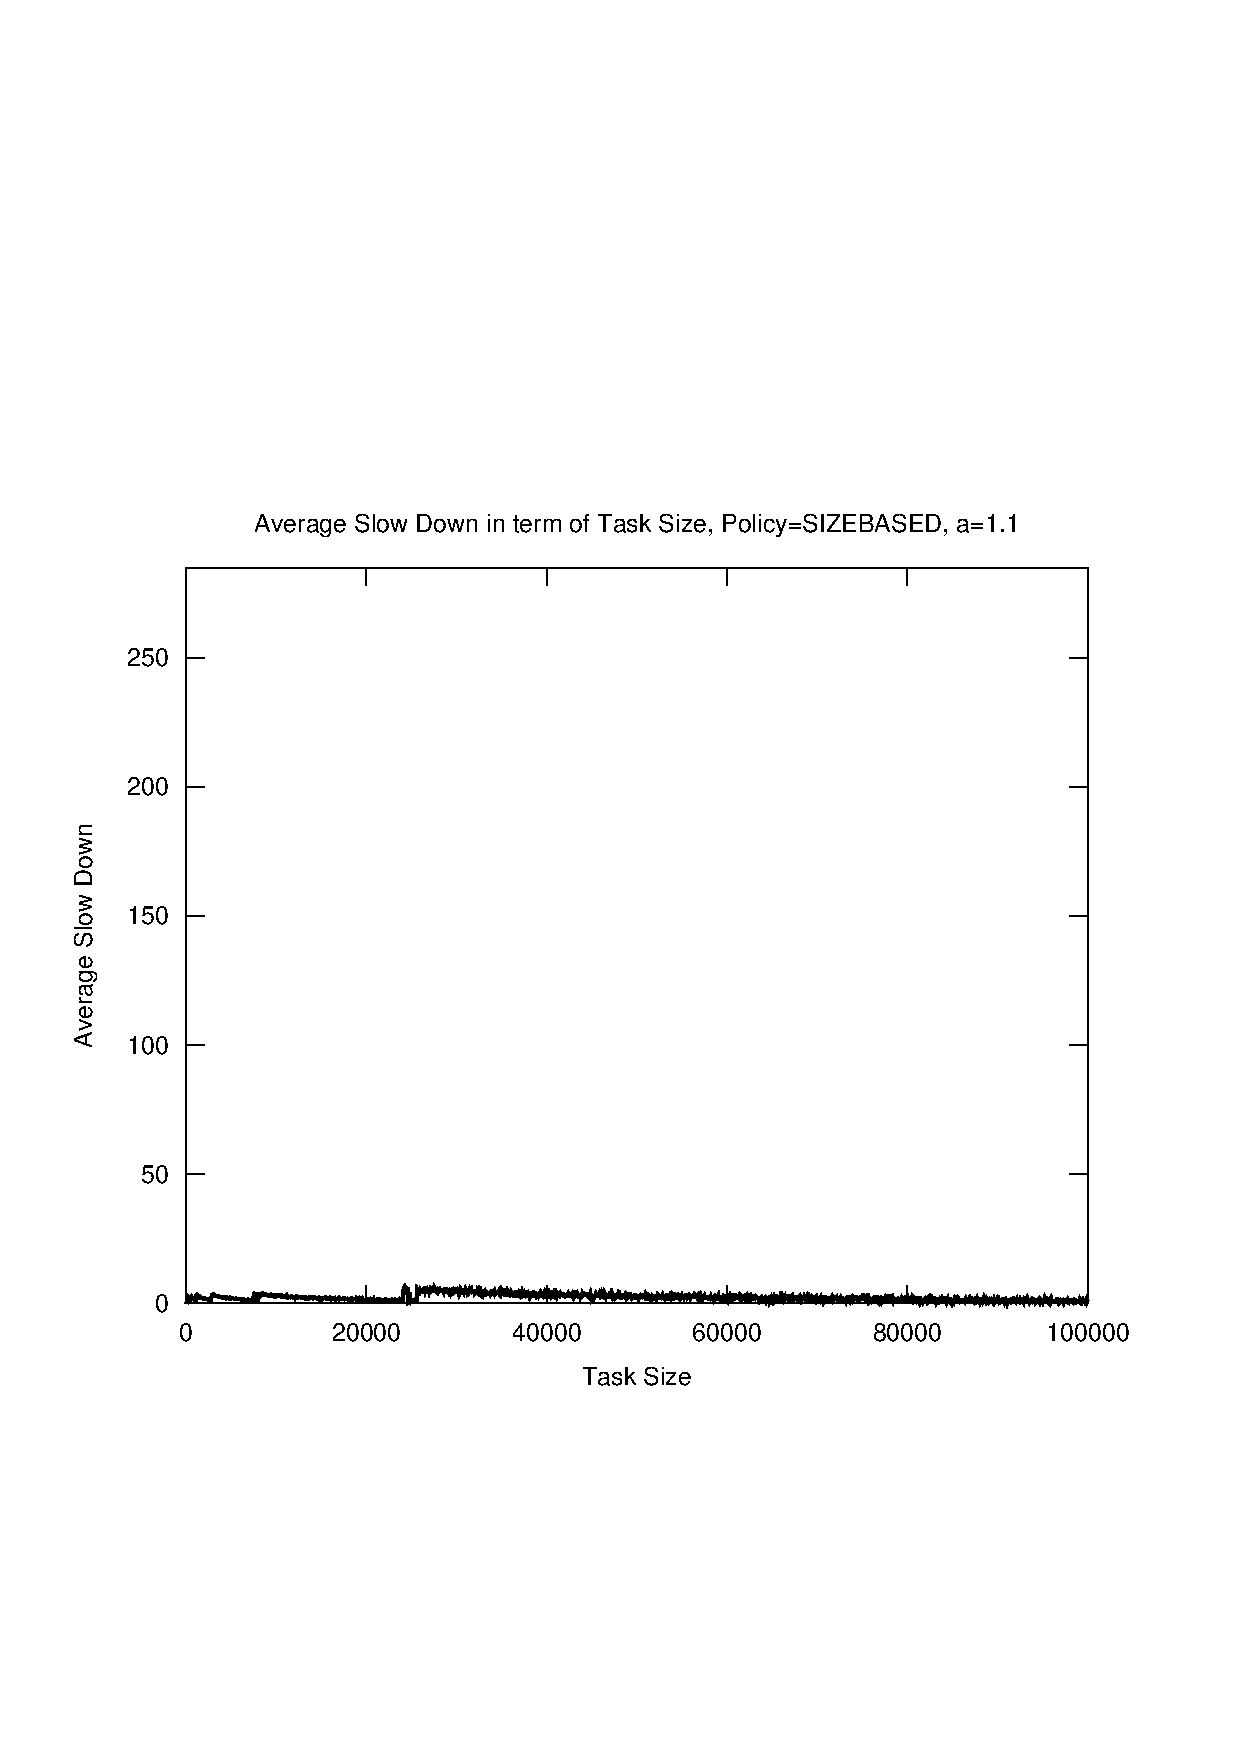
\includegraphics[scale=0.095]{alfa/graphs/binGraphs/slowDown/bin1SizeSlowDown}}
\end{frame}

\begin{frame}
	\frametitle{Average Slow Downs by Task Size, a=1.9}
	\vspace{-.1cm}
\framebox{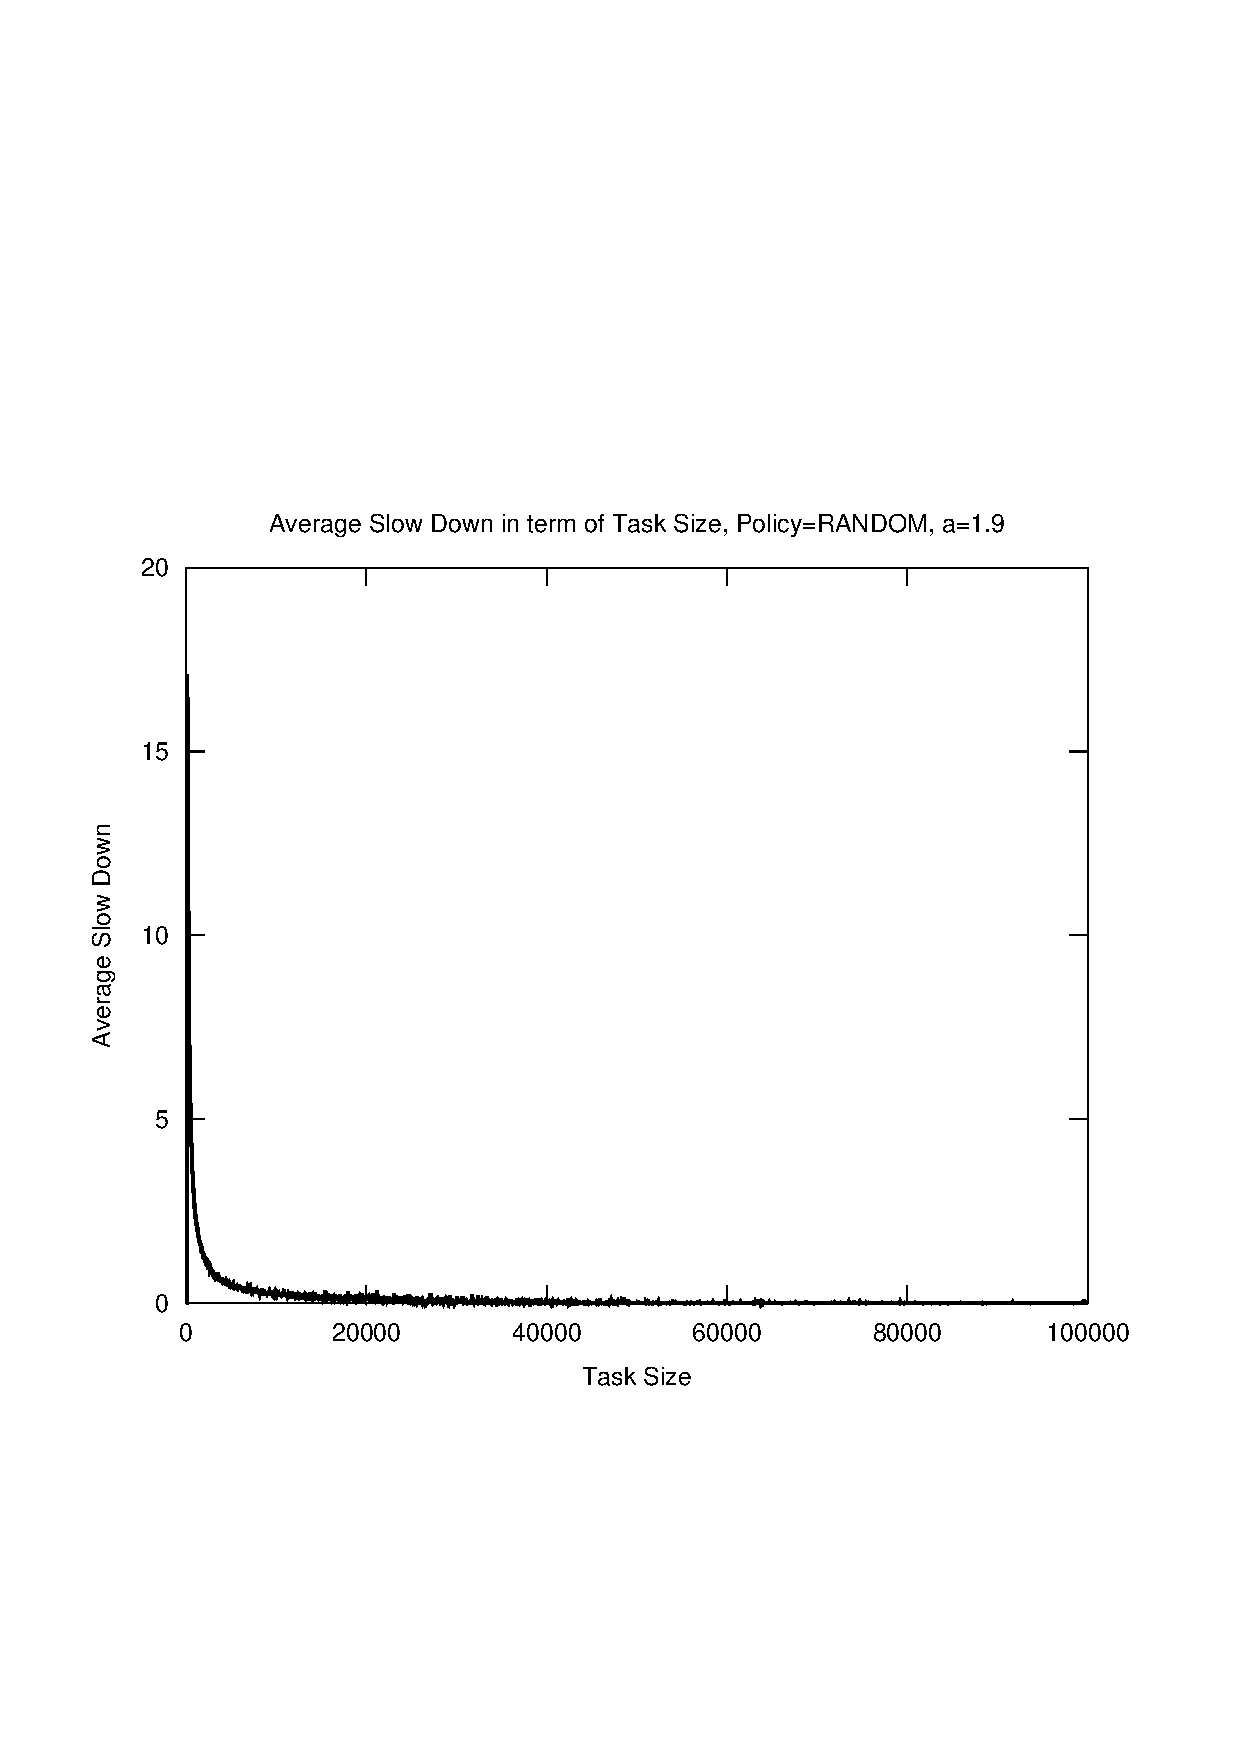
\includegraphics[scale=0.095]{alfa/graphs/binGraphs/slowDown/bin9RandomSlowDown}}
\framebox{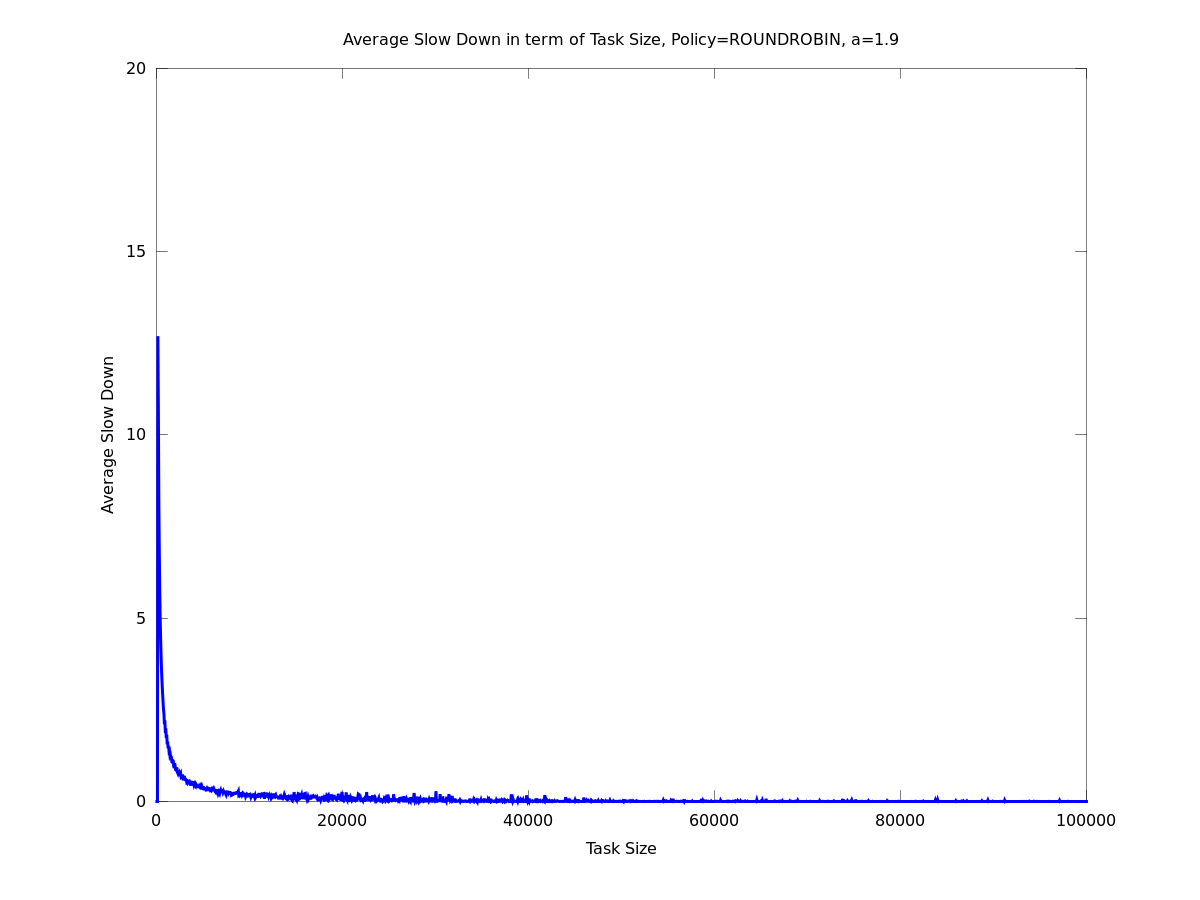
\includegraphics[scale=0.095]{alfa/graphs/binGraphs/slowDown/bin9RoundSlowDown}}	
\framebox{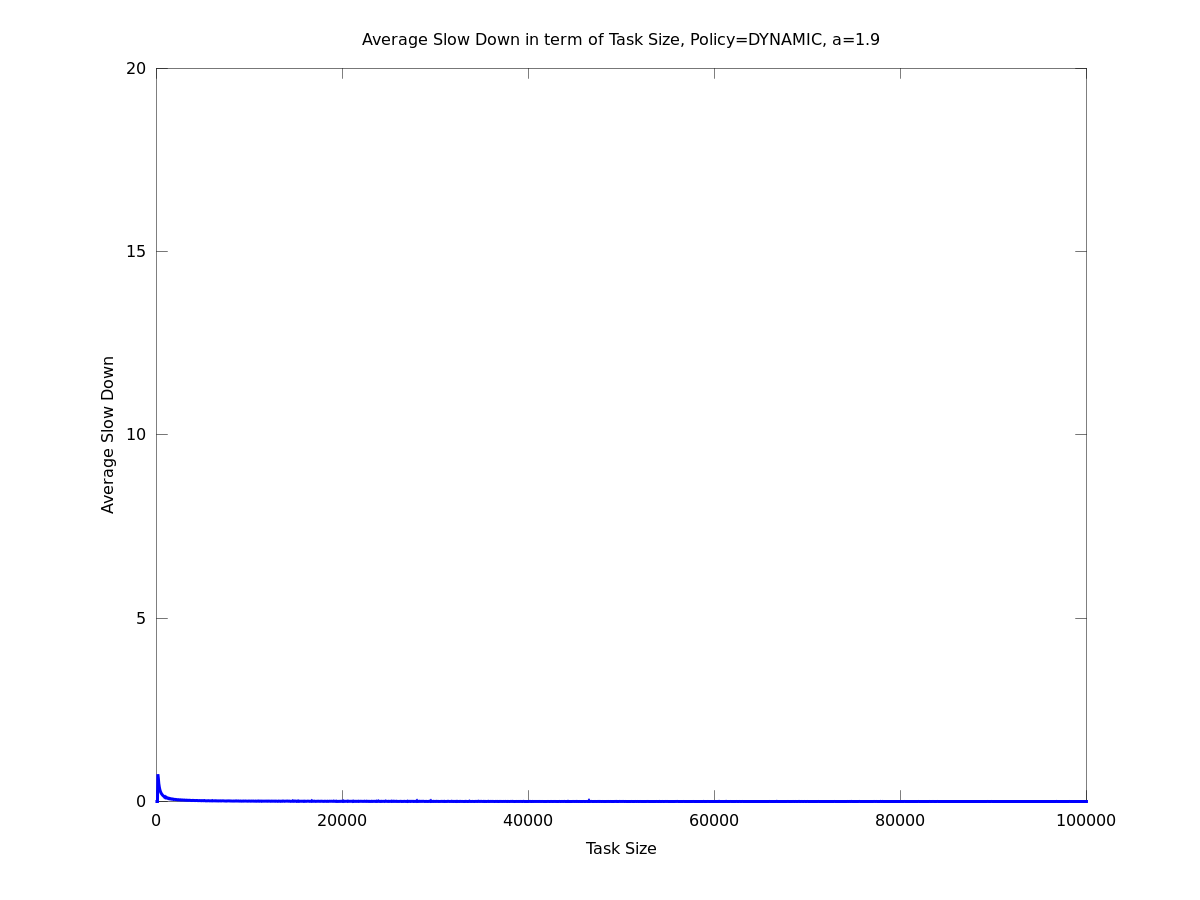
\includegraphics[scale=0.095]{alfa/graphs/binGraphs/slowDown/bin9DynamicSlowDown}}
\framebox{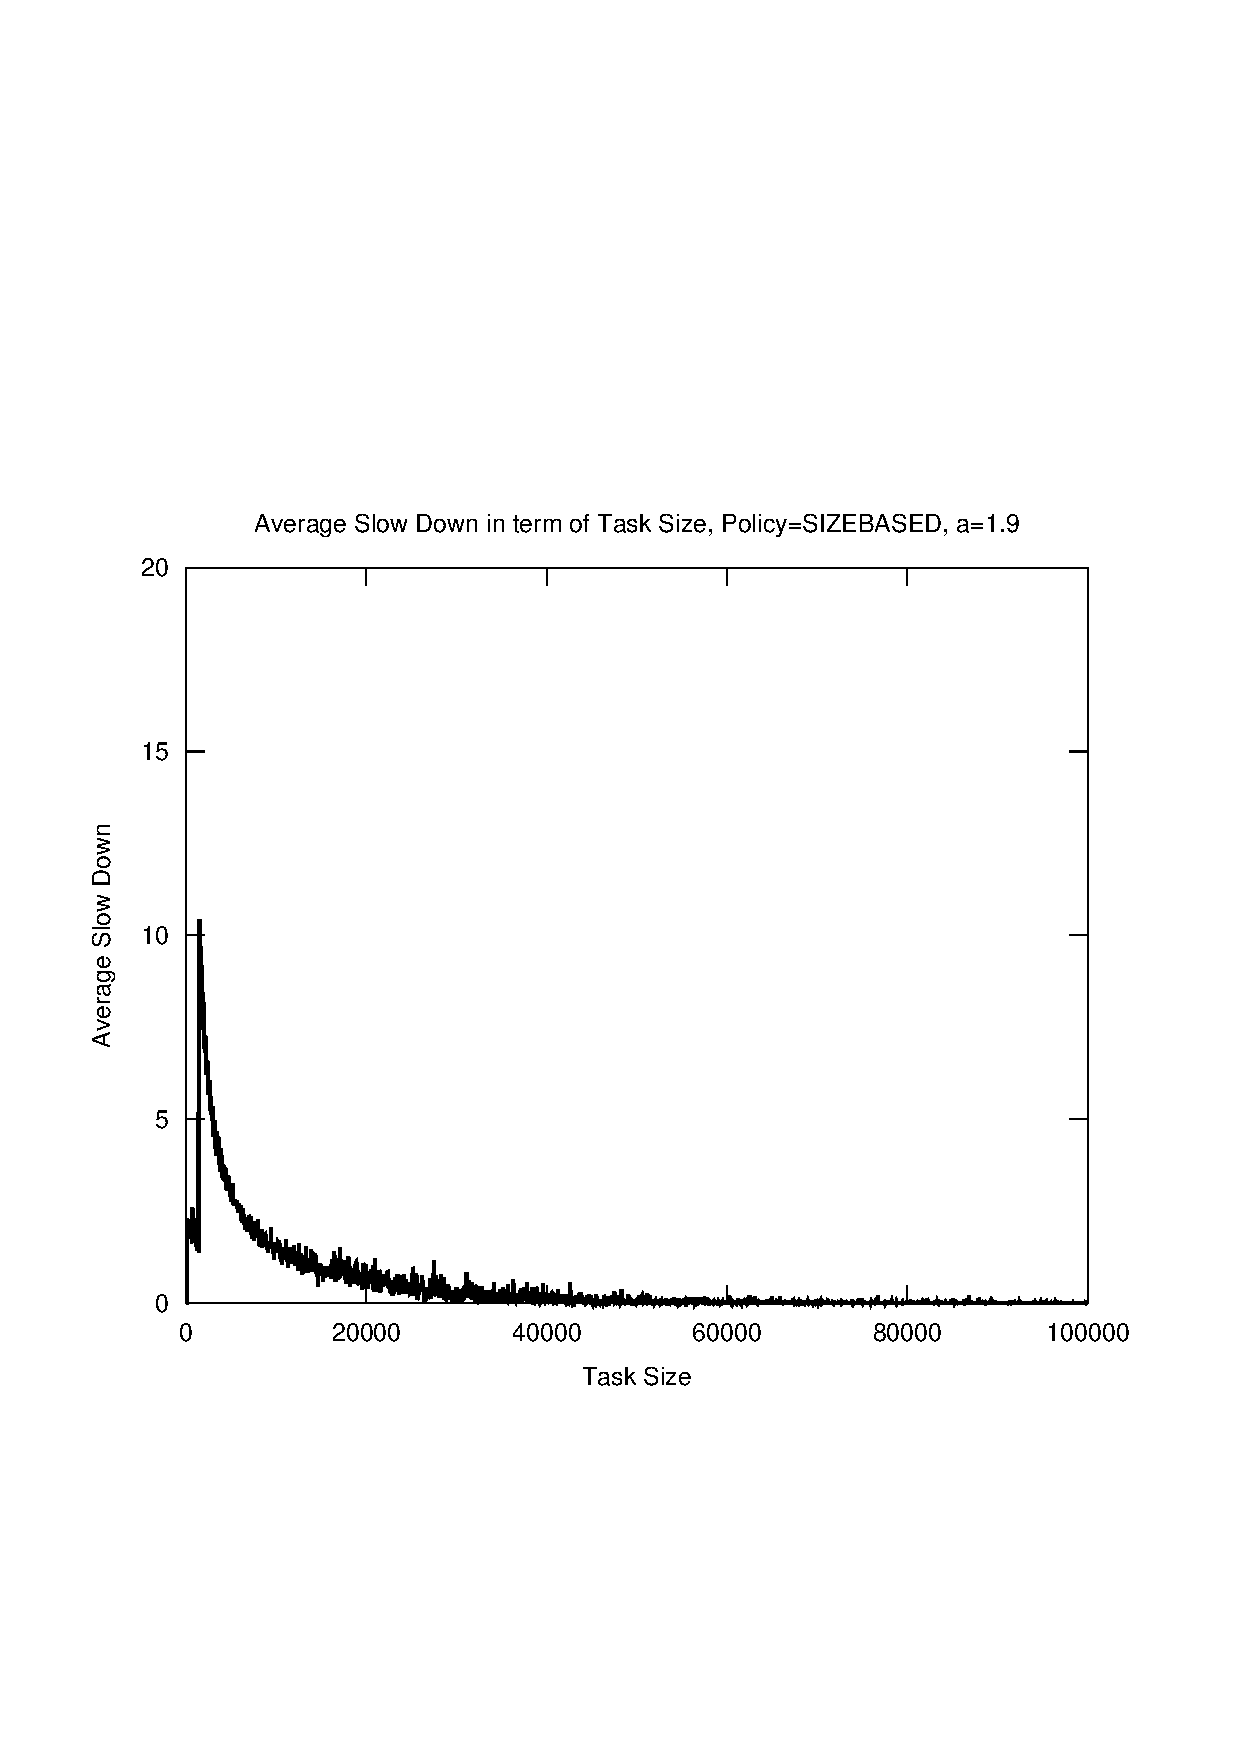
\includegraphics[scale=0.095]{alfa/graphs/binGraphs/slowDown/bin9SizeSlowDown}}
\end{frame}

\subsection{Average Queue Length Graphs}
\begin{frame}
	\frametitle{Average Queue Length - Exponential}
	\vspace{-.15cm}
	\hspace{1cm}
\framebox{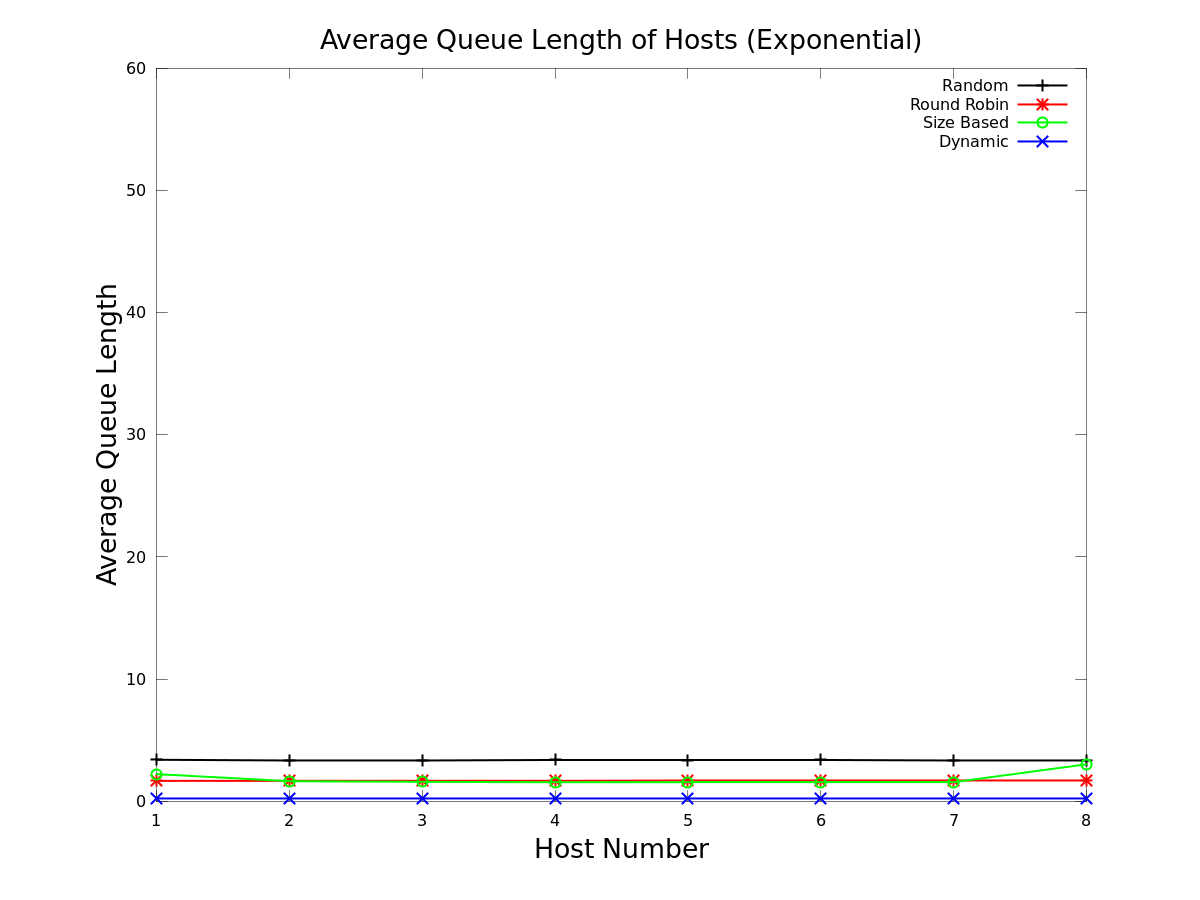
\includegraphics[scale=0.2]{alfa/graphs/aqlGraphs/exponential_aql}}
\end{frame}

\begin{frame}
	\frametitle{Average Queue Length - Pareto $a=1.1$}
	\vspace{-.15cm}
	\hspace{1cm}
\framebox{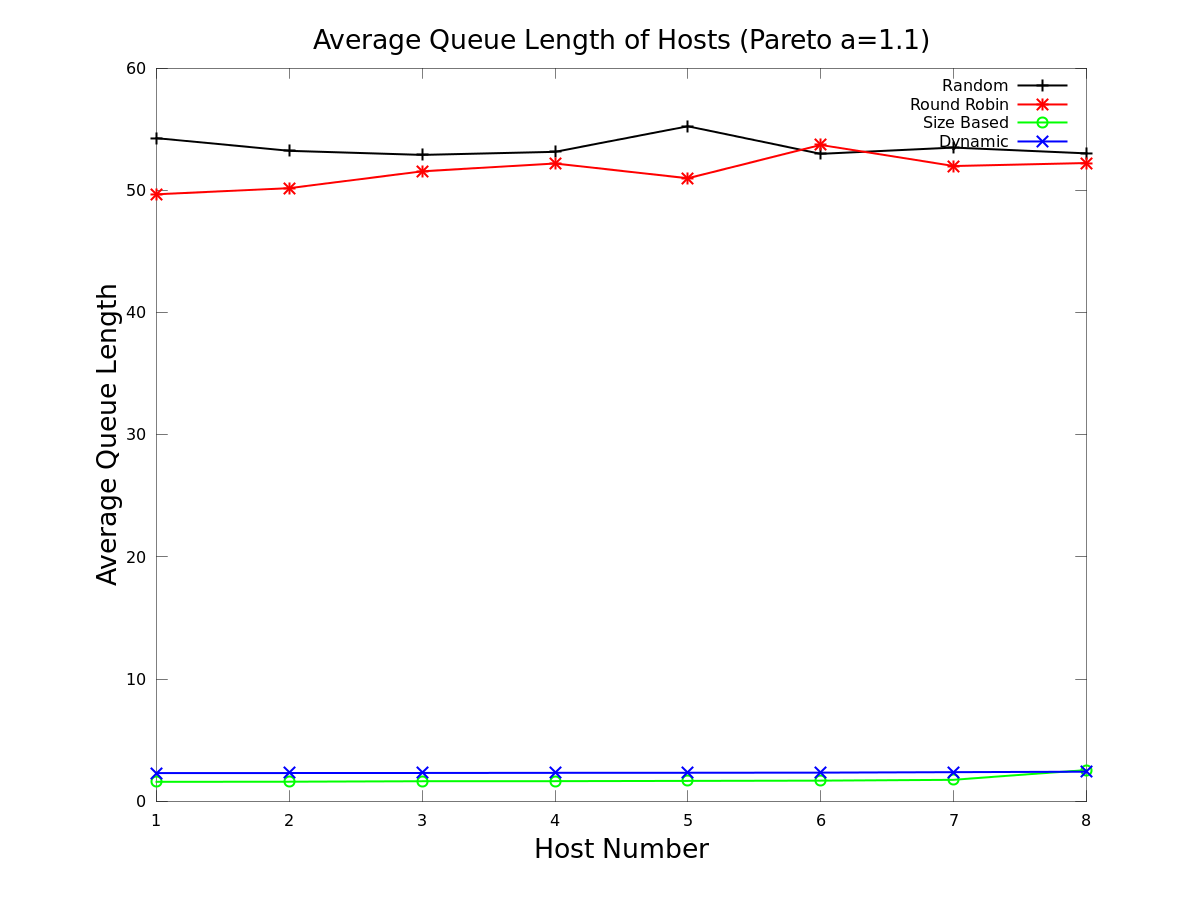
\includegraphics[scale=0.2]{alfa/graphs/aqlGraphs/pareto_1_1_aql}}
\end{frame}

\begin{frame}
	\frametitle{Average Queue Length - Pareto $a=1.9$}
	\vspace{-.15cm}
	\hspace{1cm}
\framebox{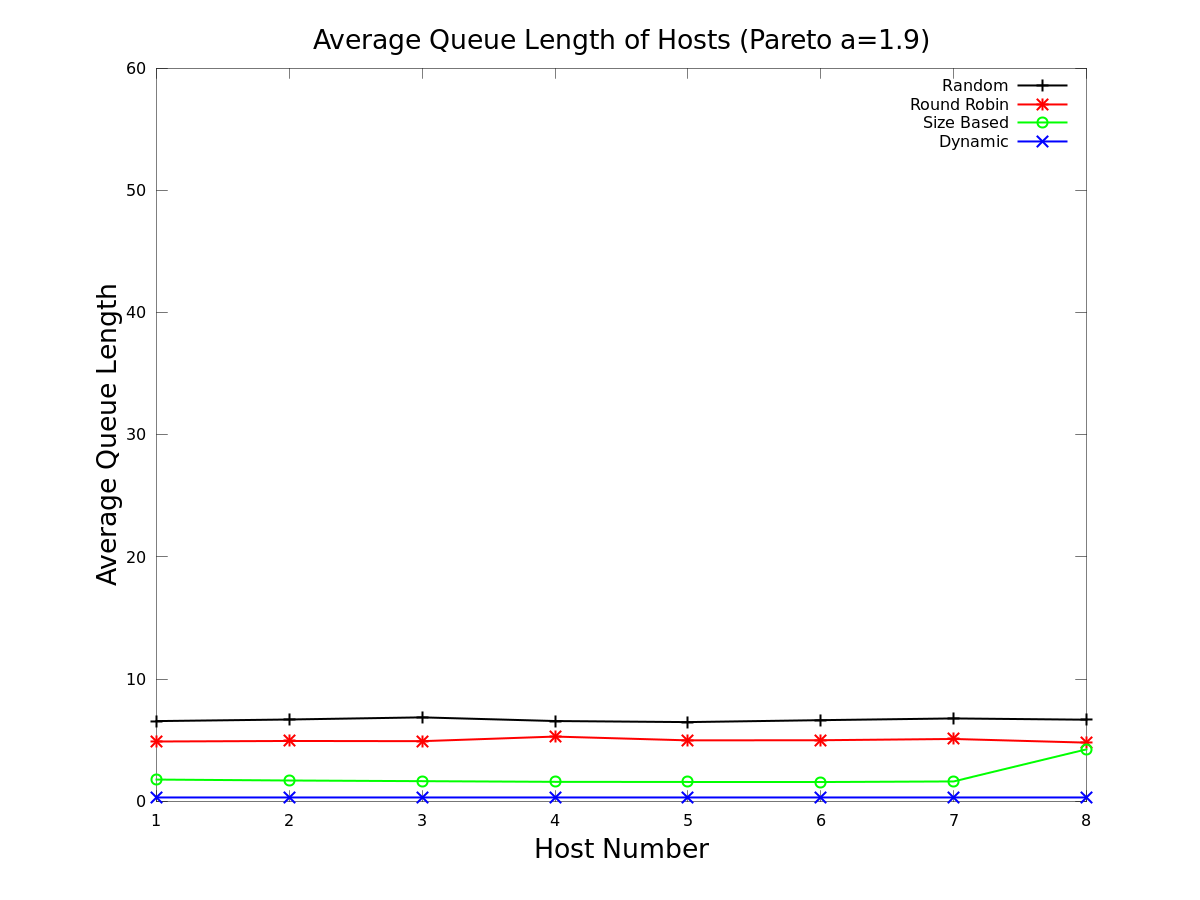
\includegraphics[scale=0.2]{alfa/graphs/aqlGraphs/pareto_1_9_aql}}
\end{frame}

\section{Conclusion}
\subsection{Findings}
\begin{frame}
	\frametitle{Conclusion}

\begin{itemize}
\item With high variance, size based policy does the best
\item While variability decreases, dynamic policy gets better
	\begin{itemize}
	\item \textit{Mathematically proofed}
	\end{itemize}
\item Size-based and dynamic always have much smaller waiting time and slowdown than random and round robin policies
\item Size based policy isn't affected a lot by variability in task size

\end{itemize}
\end{frame}

\subsection{Comparison of paper and thanks}
\begin{frame}
	\frametitle{Conclusion - Comparison of Simulation to Paper}

\begin{itemize}
\item What is done in the simulation is correlated by findings of the paper
\vspace*{2cm}
\item \textbf{\textit{Thanks for attention!}}
\end{itemize}
\end{frame}


\section{References} 
\begin{frame}
	\frametitle{References}
		
\bibliographystyle{abbrv}
\bibliography{mini_presentation}	

\end{frame}

\end{document}
